% Created 2020-02-27 Thu 17:21
% Intended LaTeX compiler: pdflatex
\documentclass[natbib,man,a4paper]{apa6}
               \usepackage{graphicx}
               \usepackage{hyperref}
\usepackage[utf8]{inputenc}
\usepackage[T1]{fontenc}
\usepackage{graphicx}
\usepackage{grffile}
\usepackage{longtable}
\usepackage{wrapfig}
\usepackage{rotating}
\usepackage[normalem]{ulem}
\usepackage{amsmath}
\usepackage{textcomp}
\usepackage{amssymb}
\usepackage{capt-of}
\usepackage{hyperref}
\usepackage{minted}
\abstract{\input{abstract.txt}}
\threeauthors{Kieran J. O'Shea}{Caitlyn R. Martin}{Dale J. Barr}
\threeaffiliations{University of Glasgow}{University of Glasgow}{University of Glasgow}
\hypersetup{colorlinks,citecolor=black,linkcolor=black,urlcolor=blue}
\authornote{Corresponding author: Kieran J. O'Shea, Institute of Neuroscience and Psychology, University of Glasgow, 62 Hillhead St., Glasgow G12 8QB; Phone +44 (0)141 330 5089.  Thanks to David Ralston and Sophie MacAskill for assistance with pilot studies, and to Holly Branigan for comments on the PhD thesis on which this article is based. Code and data are available at https://osf.io/89g5b. This work was made possible by a Doctoral Training Fellowship to Kieran J. O'Shea from the UK Economic and Social Research Council.}
\shorttitle{Ordinary memory and referential description}
\hypersetup{colorlinks,citecolor=black,linkcolor=black,urlcolor=red}
\date{\today}
\title{Ordinary memory processes in the design of referring expressions}
\hypersetup{
 pdfauthor={},
 pdftitle={Ordinary memory processes in the design of referring expressions},
 pdfkeywords={},
 pdfsubject={},
 pdfcreator={Emacs 24.5.1 (Org mode 9.0.3)}, 
 pdflang={English}}
\begin{document}

\maketitle
\begin{center}
\textbf{WORD COUNT}: 11790
\end{center}

When planning spoken referential expressions, speakers face many potential choices about what to say and how to say it. What psychological factors govern these choices? It is generally assumed that when planning messages, speakers are beholden to the cooperative principle that underlies conversational interaction \citep{grice75}. Accordingly, speakers should formulate references that convey no more and no less information than their addressee would need to identify the referent of the expression against the background of their common ground: the set of assumptions, beliefs, and knowledge that is shared, and known to be shared with their interlocutors \citep{clarkmarshall81}. Constructing expressions on the basis of this common ground---a process known as \emph{audience design} \citep{clarkmurphy82}---can help promote successful communication.  However, within the cognitive demands of real-time conversation, common ground can be too uncertain or computationally demanding to estimate and track.  It would be expected, then, that speakers take advantage of certain heuristics to make reference generation more efficient.

One such heuristic is to plan utterances relying only on information salient to the self---i.e., without first checking whether it forms part of the common ground---and to allocate cognitive resources to monitoring and adjusting the contextual appropriateness of the expression under construction \citep{hortonkeysar96}.  For instance, a speaker might generate a plan to refer to a candle as \emph{the small candle} to distinguish it from a larger one she knows about, or because she is relying on a referential precedent (or `conceptual pact') established earlier in the discourse \citep{brennanclark96}.  She may rely on the knowledge of the larger circle or the existing precedent simply because they are available during the message generation process \citep{DellBrown1991}, not necessarily because they are part of common ground with the addressee.  Using common ground may require considerable time and cognitive resources \citep{hortonkeysar96,rossnagel00}, which can be in short supply in real-time conversation. This \emph{perspective adjustment} strategy of egocentric planning while using common ground during self-monitoring \citep{hortonkeysar96} compromises accuracy for efficiency, but may be effective under the assumption that interaction brings interlocutors' perspectives into alignment \citep{pickeringgarrod04}. Moreover, relying on egocentrically available information may not be a huge risk since communicative situations allow for the collaborative detection and resolution of miscommunication \citep{fussellkrauss92}.  

Supporting this view, egocentrically-available information reliably impacts production on a variety of levels, including for example reference generation \citep{wardlowlanegroismanferreira06}, syntax \citep{ferreiradell00}, and the use of pronouns \citep{FukumuraVanGompel2012}. But what exactly is this `egocentric' information, how does it become accessible in the first place? In theoretical discussions, egocentric information is often defined negatively---as whatever cannot reasonably be considered as part of common ground. Unpacking what representations and processes are responsible for making information available in a timely fashion should be an important goal for any theory of language production.

One appealing possibility is that availability is determined by ordinary processes of memory encoding and retrieval.  This \emph{ordinary memory view} \citep{hortongerrig05} assumes that everyday memory processes can serve as a proxy for common ground, activating potentially relevant information naturally and effortlessly through cue-driven, parallel search processes often characterized in terms of ``resonance'' \citep[e.g.,][]{hintzman86}.  

Consider a speaker who wishes to refer to referent \(R\) (e.g., a candle) in context \(C\) (e.g., the speaker's living room, while speaking to a friend) and finds it necessary to use expression \(E\) (e.g., ``the small candle'') which includes the modifier `small' because of features of the context (e.g., the presence of a larger candle).  Models of expertise and skill development \citep{logan88,loganetherton94} suggest that constructing an expression for \(R\) will at first be done `algorithmically'---that is, through deliberative mechanisms involved in everyday problem solving. The cognitive operations and representations involved in this initial assembly become stored in memory as an episodic trace: a \emph{processing episode} \citep{logan88}. With repetition, the process of generating an expression will become increasingly automatized---specifically, the production process will increasingly rely on the wholesale retrieval of expression \(E\) from memory on the basis of \(R\) and \(C\), which act as retrieval cues. To the extent speakers attend to features of the communicative context during this process (e.g., the environment and audience), these features will become part of the stored processing episode that link the problem situation (i.e., referring to \(R\) in context \(C\)) to the output solution (the expression \(E\)), with each repetition strengthening these links.

Such a view of message generation takes advantage of the key memory principle of \emph{encoding specificity}: stored information becomes available in proportion to the the overlap between encoding and retrieval environments \citep{tulvingthomson73}.  The retrieval process may activate various candidate expressions that the speaker has used for the same or similar targets in the past (e.g., ``the candle'', ``the red candle'', ``the small candle'').  Following this principle, the extent to which various candidates are activated will depend on the similarity between the current communicative situation and past situations in which these expressions have been used, providing a kind of automatic route for speakers to produce contextually appropriate references. 

Insomuch as similar situations require similar referential expressions, ordinary memory processes may offer a shortcut to successful communication, enacting a process referred to as \emph{attribute substitution} in the judgment and decision-making literature \citep{KahnemanFrederick2002}.  Attribute substitution is likely to occur whenever a \emph{target attribute} that is needed for a judgment is effortful to compute and there is a \emph{heuristic attribute} available that is correlated with the target attribute, allowing the decision maker to use the latter as a proxy for the former.  In the case of reference generation, prior theorizing suggests that the strength of a memory signal associated with a particular referring expression could be a heuristic attribute that can be substituted for the target attribute of common ground.  When the speaker attends to a referent with a referential goal, various candidate expressions would become available through memory resonance processes, and the speaker could assess their relative appropriateness in the context through their relative activation strengths \citep{GannBarr2014}.  Similarly, \citet{horton_gerrig_2016} propose that during early stages of utterance generation, retrieval strength could provide a primitive form of \emph{commonality assessment}, with strength of activation providing a surrogate for more explicit computation of common ground.

To the extent that memory associations correlate with common ground, ordinary memory processes could make communicatively relevant information available at minimal cognitive cost.  A key prediction of the memory-based view is that conversational partners themselves can act as memory cues, such that the perceptual experiences arising through interactions with a given partner (e.g., the quality of their voice, their appearance, or interaction style) become associated with information that has been shared during those interactions, such that each encounter with the interaction partner re-instantiates shared information.

Although the ordinary memory view has been influential, there is currently little understanding of how, and how much, ordinary memory processes impact information selection during reference generation. Much of the existing support for the view is indirect: for instance, \cite{hortongerrig05} demonstrated that factors affecting memory encoding also impact reference generation, implicating memory as an underlying mechanism. In a picture naming study, speakers were faster to name pictures when speaking to the same partner than when speaking to a different partner \citep{horton07}. This suggests that speakers not only associated previously-produced descriptions with pictures, but also with the prevailing context, including information about the identity of the addressee. However, a later replication attempt called this finding into question \citep{brown-schmidt_horton_2014}. But even assuming the original effect is real, showing enhancement of a performance aspect of production (speech onset time) would fall short of supporting the most important claim of the ordinary memory account for production: that ordinary memory processes can stand in for common ground in the determination of the informational content of an expression.

Ordinary memory can be an effective proxy for common ground for message generation only if two conditions are met: (1) people retain detailed information from previous referring episodes, and (2) these detailed memory representations are accessible to, and taken into account during, the information selection process. The first assumption is well-supported by a large priming literature indicating that people do retain detailed information from past episodes that can influence future behavior, even after long delays \citep{tulving_schachter_1990}.  However, it is possible that these types of priming processes operate somewhat independently of message planning, influencing aspects of performance (such as speech onset latency) but wielding little or no impact on the selection of information.  Thus, it is critical to assess not only the presence of these largely implicit factors, but also to measure their impact on the informational content of speakers' references. These are the main goals of the present set of studies.

\subsection*{Overview of Experiments 1--3}
\label{sec:org48f44ba}

Following work by \cite{brennanclark96} and \cite{GannBarr2014}, the logic of the current investigation was to entrain speakers on a referential expression \(E\) for referent \(R\) in training context \(C\), and then to measure aspects of production in a test context \(C'\) that required a different expression, \(E'\). For example, in the training context a speaker might refer to a particular \(R\) using expression \(E\), ``the small candle'', to distinguish it from another larger candle in the referential array. Later this same candle would appear in a test context \(C'\) where the larger candle was absent.  When speakers in \(C'\) call the referent ``the small candle'' (\(E\)) instead of simply ``the candle'' (\(E'\)) they do so because they are relying on memory instead of the information available in the display. Because we are interested in memory effects, the misspecification rate in \(C'\) provides the critical data for our study.

To obtain direct evidence for the ordinary memory view, our study goes beyond previous studies by varying not only the informational requirements from \(C\) to \(C'\), but also perceptual characteristics that could affect memory retrieval independently of common ground. To the extent ordinary memory processes influence information selection, speakers should be increasingly likely to retrieve \(E\) in the test context \(C'\) as a direct function of the perceptual similarity between \(C'\) and the training context \(C\), leading in turn to a higher misspecification rate. This key prediction of the ordinary memory view falls out of the encoding specificity principle \citep{tulvingthomson73}: similarity between encoding and retrieval contexts facilitates retrieval. 

To test this prediction, we used the following basic paradigm. Across three experiments, speakers and addressees sat at separate computer screens and engaged in referential communication about shared images.  This made it possible to change features of the speaker's display between training and test independently of the addressee's display. In the first two experiments, we varied the similarity in the the physical arrangement of images between training and test.  In the context of these experiments, the position of a referent on the display was communicatively irrelevant, since speakers believed that listeners viewed a different arrangement of the same objects. In both of these experiments, in addition to recording speakers' descriptions, we also measured their implicit memories for the training displays by tracking eye movements at test. While the implicit measures suggest retention of training display information, there was little evidence for any impact of these implicit memories on speakers' tendency to re-use the descriptions acquired during training.

In the third experiment, speakers spoke to two separate addressees over a video link, which allowed us to manipulate which partner appeared on the screen independently from which partner they were actually speaking to. On certain test trials, speakers viewed a video feed of a partner to whom they had been speaking during training, although they were aware that they were in fact speaking to an addressee who remained off-screen. By independently manipulating who the speaker saw from who they were actually speaking to, we directly tested the idea that partners can serve as a memory cue during message generation. We also independently measured whether speakers kept track of common ground. Although speakers' descriptions were influenced by the identity of the addressee, there was little evidence that the partner they looked at influenced the content of their speech.

The methods and analysis protocols for all three experiments were pre-registered at the Open Science Framework (OSF).  The master repository for this project is available at \url{https://osf.io/89g5b}, which includes links to pre-registration documents for each experiment, as well as data, code, and a software container providing all necessary infrastructure to reproduce our findings.

\section*{Experiment 1}
\label{sec:orgc18e05b}

\begin{figure}[htbp]
\centering
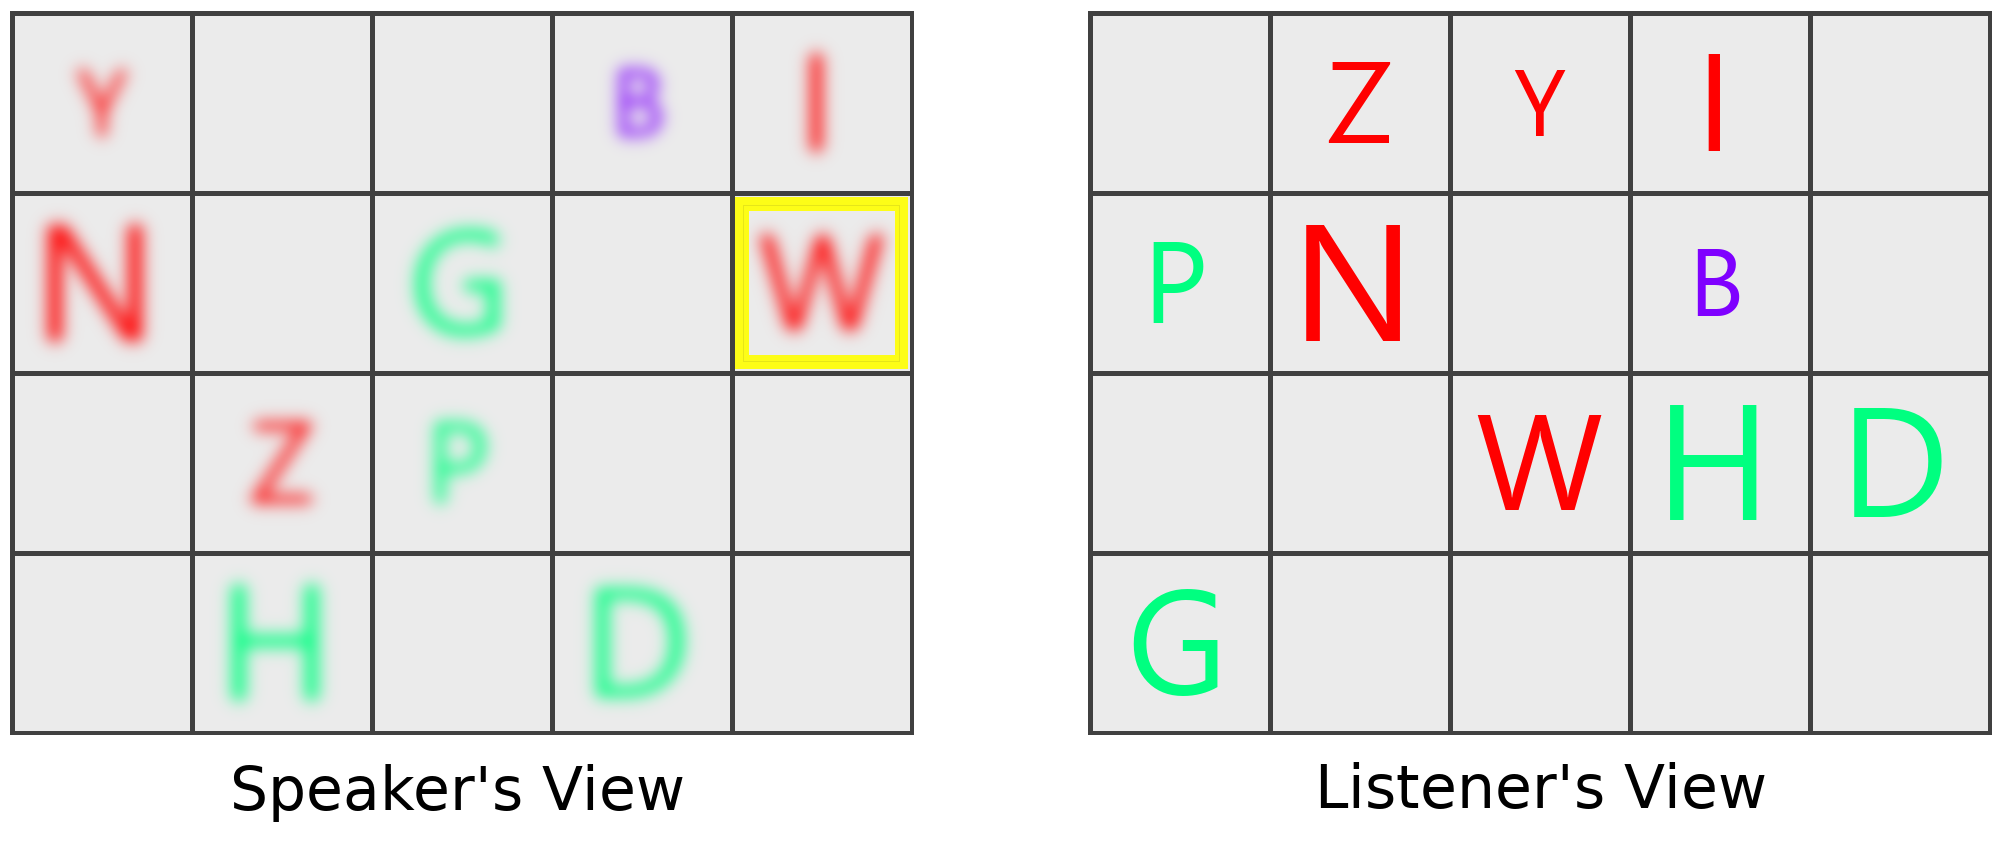
\includegraphics[width=.9\linewidth]{figs/Exp1.png}
\caption{\label{fig:org4dd7000}
Example test trial displays for Experiment 1 from the Contrast-Singleton condition. The target letter (W) is surrounded by a yellow highlight. The foil letter (Y) appears in the upper left square of the Speaker's view. Note that the Speaker's display was deliberately blurred to make it more difficult to use peripheral vision.}
\end{figure}

In Experiment 1, speakers referred to capital letters of the alphabet in displays containing multiple distractor letters varying in size and color (Figure~\ref{fig:org4dd7000}). Following previous experiments \citep{brennanclark96,GannBarr2014}, we induced referential overspecification using \emph{training} and \emph{test} trials with different informational requirements. For example, during training, a speaker might refer to the letter `W' as ``the large W'' to distinguish it from a smaller-sized `W' in the same array. In the corresponding test trial, the smaller \emph{competitor} W would be replaced by a \emph{foil} letter---a letter with a different identity but that was visually similar to W (e.g., Y) and that also had the same color and size as the competitor (as shown in Figure~\ref{fig:org4dd7000}). For all targets in the experiment, size was the only dimension distinguishing the target from the competitor.

We refer to this condition, where the target (e.g., `W') appeared in training as part of a contrast including a smaller `W' and as a singleton on the test trial, as the  \emph{Contrast-Singleton} condition. To the extent speakers rely on their memory of the training trials, they should overspecify the target at test. Also---and, departing from previous experiments---we included a \emph{Singleton-Contrast} condition intended to induce speakers to \emph{underspecify} referents. In this condition, the target letter appeared as a singleton during training (i.e., with the foil) leading speakers to entrain on the base noun (``the W''), while at test the same target would appear as part of a size contrast with a letter of the same category. If speakers continued using the base description at test, they would provide too little information for the listener to identify the referent.  Together, these two conditions formed the levels of a single within-participant factor, \emph{Shift Direction}.

\begin{figure}[htbp]
\centering
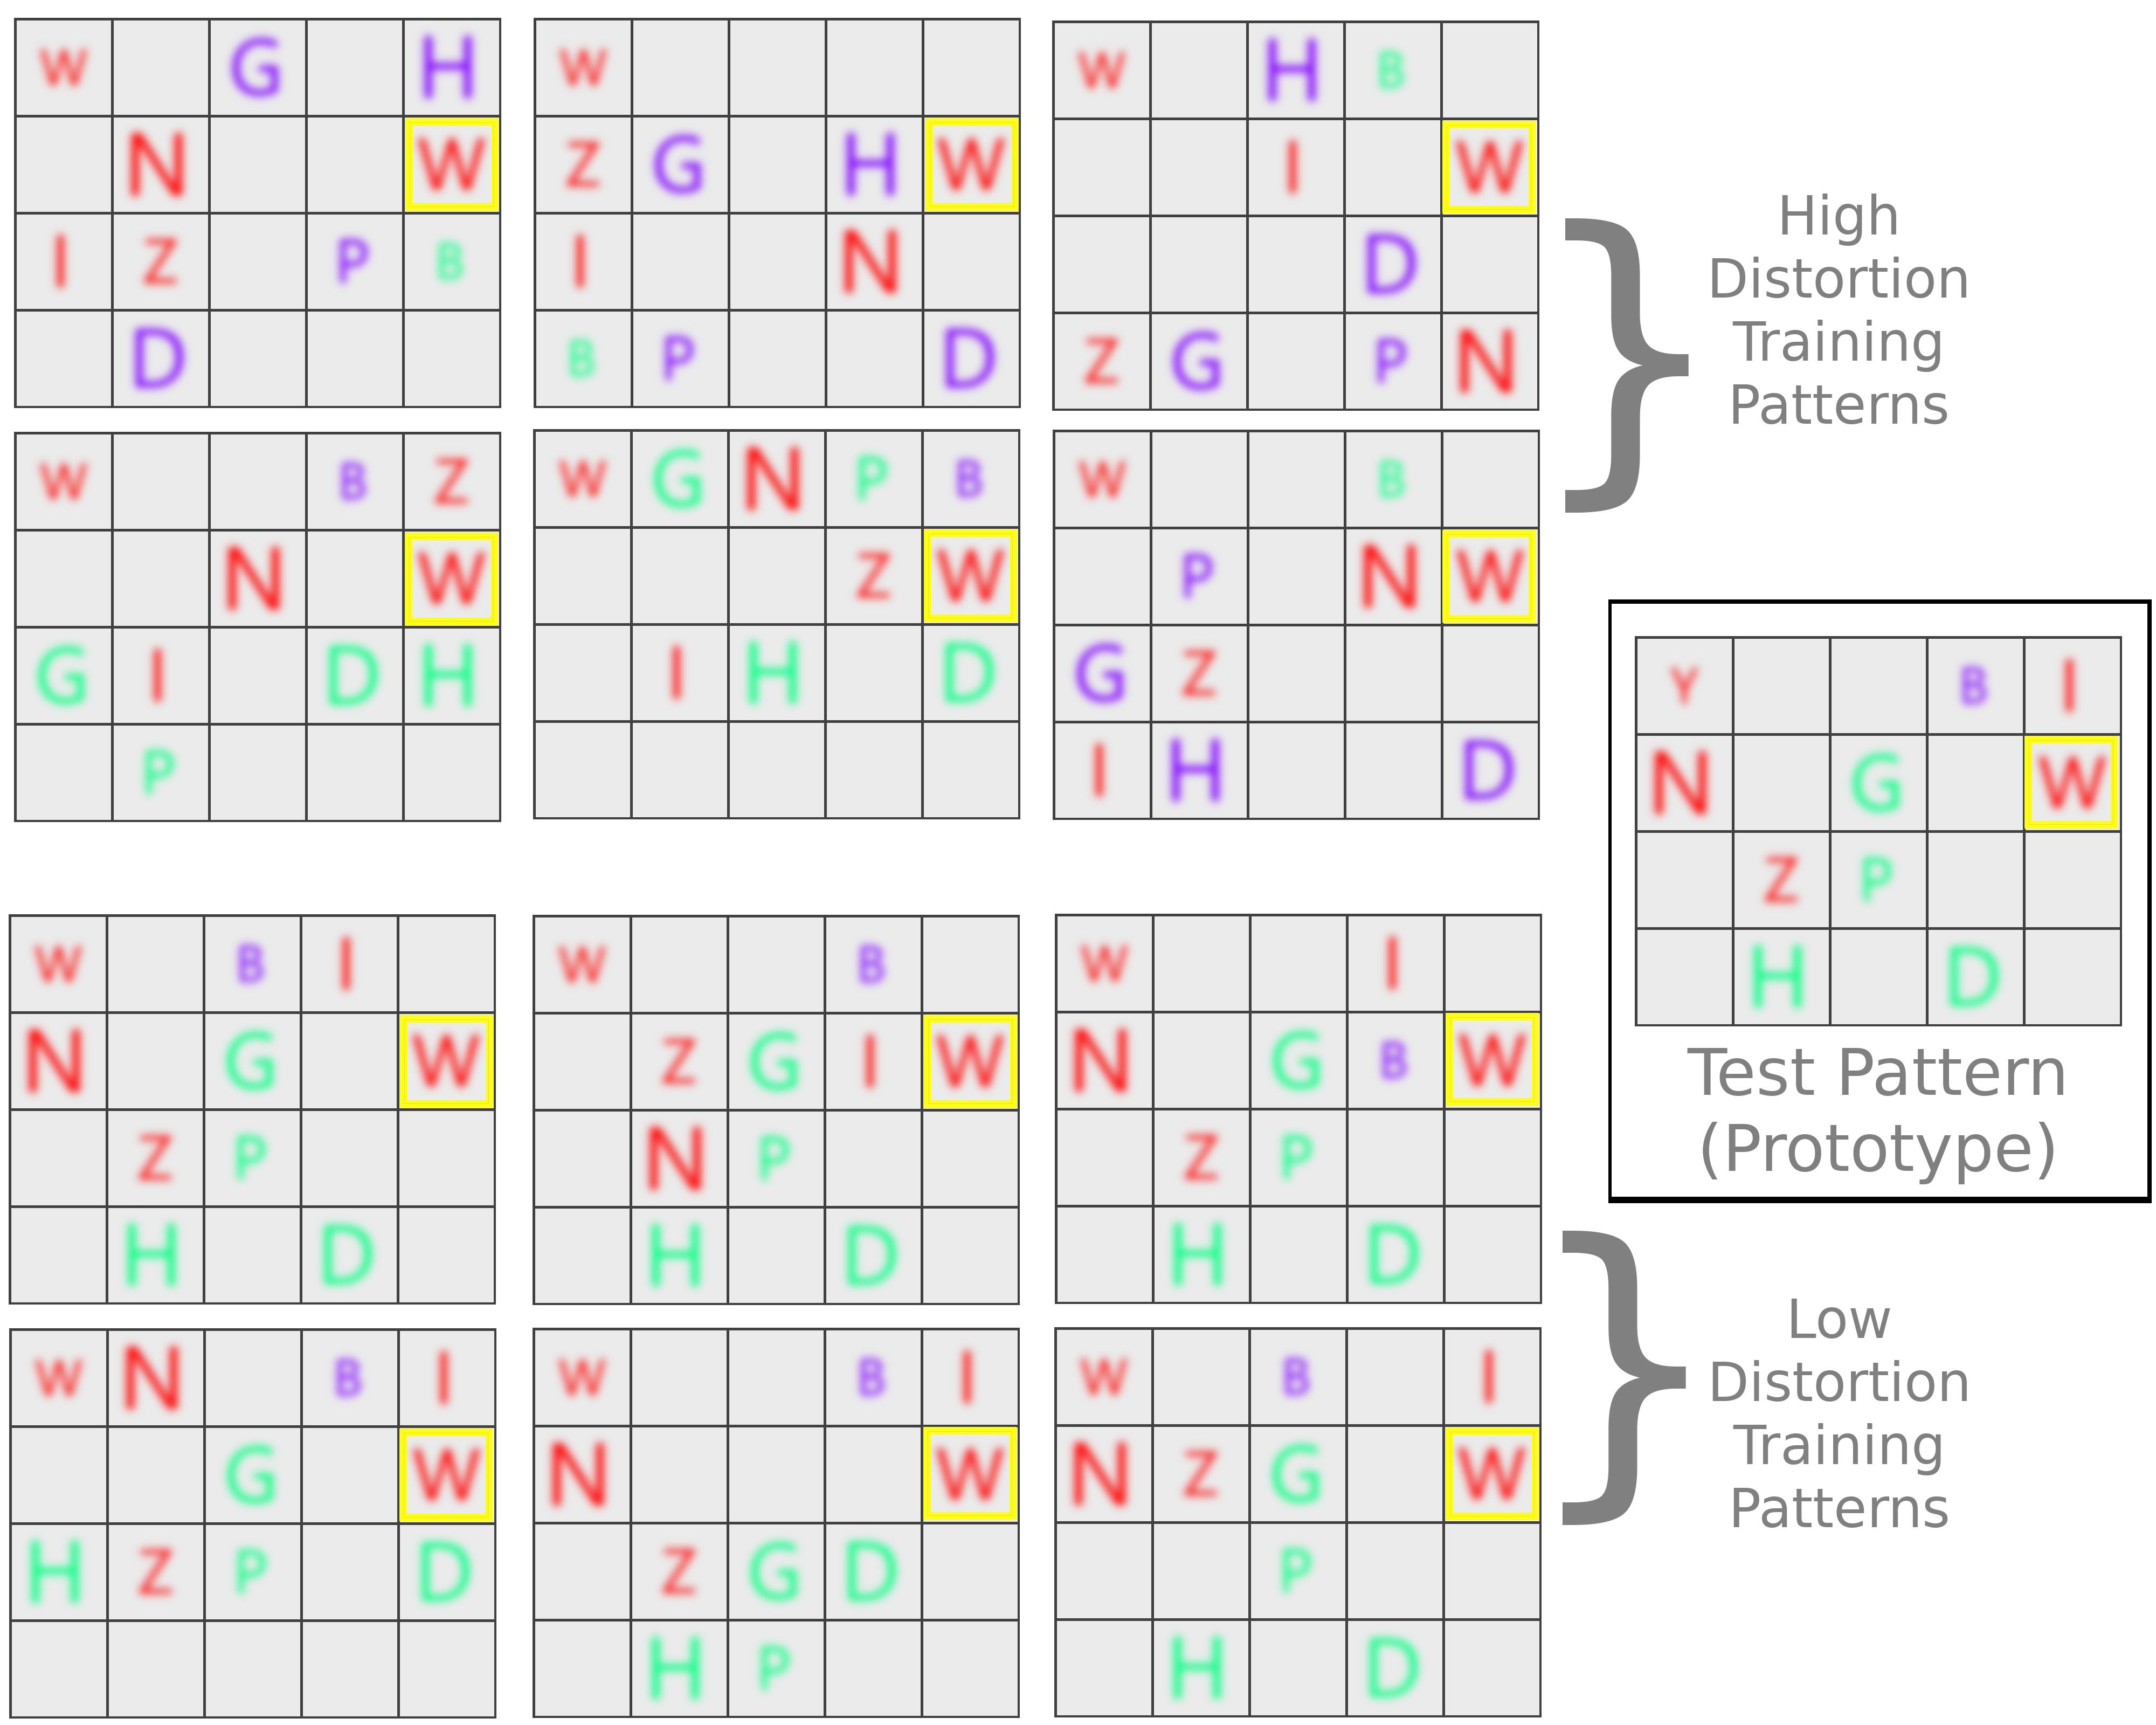
\includegraphics[width=.9\linewidth]{figs/Exp1_HvL.png}
\caption{\label{fig:orgcaa0713}
Example prototype with six distortion patterns in each of the two conditions, Experiment 1.}
\end{figure}

The critical question in this study was the extent to which the misspecification of target letters varied as a function of the perceptual similarity between the training and test trials. The position of letters in the array was never communicatively relevant, because speakers knew that the listener viewed the same letters, but in a different, unknown arrangement. To test the ordinary memory account, we randomly generated test grids to use as prototypes, which we spatially distorted to create the training trials (Figure~\ref{fig:orgcaa0713}), as in the classic memory study by \cite{posner_keele_1968}. There were two levels of the within-subject factor of \emph{Distortion}: \emph{Low Distortion}, where the training trials were highly spatially similar to the test prototype; and \emph{High Distortion}, they were less spatially similar to the prototype. To the extent ordinary memory processes influence information selection, speakers in the \emph{Low Distortion} condition should be more likely to misspecify referents, because the association between the test display, the referent, and the expression used at training should be stronger and thus more likely to be retrieved.

We chose spatial arrangement as a memory cue because it is widely known that people retain episodic traces of spatial configurations, and that such traces influence aspects of processing; for instance, people are faster to locate a search target when the display configuration is similar to a previous trial \citep{chun_jiang_1998}.  Similarly, when viewing familiar scenes, people scan them differently, sampling familiar elements less frequently \citep{ryan2000amnesia}.  We also used it as a cue because we could easily measure memory for spatial configuration using eyetracking. Because the test display is the prototype of the distortions viewed during training, it should seem more familiar to speakers in the \emph{Low Distortion} condition, and we should expect different scanning patterns relative to the \emph{High Distortion} condition. To the extent we find these differences without changes in speakers' misspecification rate, this would suggest that implicit memory may operate somewhat independently from message planning.

Our main pre-registered prediction was that speakers would be more likely to misspecify referents in the \emph{Low Distortion} than in the \emph{High Distortion} condition. We also predicted that it would take speakers longer to produce appropriately specified descriptions in the \emph{Low Distortion} condition. We also included two predictions of secondary importance: (1) that speakers would be more likely to overspecify than to underspecify targets; and (2) that speakers would gaze at fewer non-target items prior to speech onset in the \emph{Low Distortion} condition. In the end, we opted for a more comprehensive time-series approach to analyzing the eye data, and so the eye-tracking results for the pre-registered hypothesis are reported as part of the online materials.

\subsection*{Method}
\label{sec:orge0b5ac0}

A link to the pre-registration for this experiment can be found in the OSF repository.

\subsubsection*{Participants}
\label{sec:orgdb5993b}

We collected data from a a total of 47 participants, with data from 11 excluded for reasons specified below, leaving 36 participants included in the analysis. The participants were 24 women and 12 men. The sample size of 36 was determined in advance, through a power analysis based on a small pilot study (80\% power for the effect observed in the pilot). All participants were recruited from the University of Glasgow campus and were either paid £6 or received course credit.

From our pilot study, we were concerned that some speakers would opt for a strategy of overdescription---that is, always using a size modifier even when there was not a competitor letter in the display. The problem with this behaviour is that on test trials in the \emph{Singleton-Contrast} condition, speakers could simply continue using the modified description, which would then spuriously appear to be appropriately specified. We pre-registered our intent to exclude any participants who inappropriately used size modifiers on more than half of the the final training trials for each sequence in the \emph{Singleton-Contrast} level. This resulted in the exclusion of ten participants. One additional participant was replaced due to a problem that we did not anticipate in our pre-registration protocol. This speaker used excessively long descriptions on each trial, seeming to have misconstrued the task as one of providing fine-grained description rather than providing sufficient information for the experimenter to locate the target.

Subjects gave written informed consent before beginning the experiment and were fully debriefed after the experiment had finished. Our procedures fully complied with the ethical code of conduct of the British Psychological Association.

\subsubsection*{Experimental Setup and Task}
\label{sec:org2582c87}

The experiment was interactive with the participant playing the role of speaker and the experimenter playing the role of the listener. The speaker and the listener sat in different areas of the testing room and looked at separate computer monitors throughout the experiment. Both were seated facing in opposite directions so that they were unable to see the other's display. In each trial, the speaker was asked to describe a highlighted target letter, which appeared on their monitor, to the listener. The listener then identified this letter on his own screen and selected it using a computer mouse. The target letter appeared on the speaker’s screen within a grid among other distractor letters (Figure~\ref{fig:org4dd7000}). The speaker was informed that in each trial the listener would have the same letters on their monitor but that they may be arranged in a different format compared to the grid that appeared on their screen.

\subsubsection*{Design}
\label{sec:orgc529c3c}

There were two factors in the design, \emph{Distortion} (\emph{Low}, \emph{High}) and \emph{Shift Direction} (\emph{Singleton-Contrast} and \emph{Contrast-Singleton}), forming a full-factorial 2x2 within-participant design.

\subsubsection*{Materials}
\label{sec:org75c04bf}

Each display consisted of a five-by-four grid containing uppercase letters (A-Z) of different font size and colour. All letters appeared in uppercase Arial font. The font sizes for targets and competitors/foils were randomly generated for each trial, with `small' defined as between 64--96pts and `large' as 32pts higher than the smaller letter in a pair.  We refer to a single `sequence' as the set of training trials and the single test trial associated with a single target-competitor-foil triad. There were 48 sequences in each experimental session. Displays and target/foil pairs were randomly generated for each participant. For each sequence, the number of training trials was randomly chosen from a range of 6 to 9. Given these parameters, each experimental session could have contained anywhere between 336 trials (6 \(\times\) 48 training trials plus 48 test trials) and 480 trials (9 \(\times\) 48 training trials plus 48 test trials).  

Each sequence for each session was based on a randomly generated original ``prototype'' display, which was used as the test trial, with the training displays generated as distortions of this prototype.  The identity, color, and size of the target letter in each sequence were fixed across all displays. The identity of the target letter was chosen randomly for each sequence in each session, with the constraint that the same letter could not be used as target more than once per session within each block of 24 sequences formed by the \emph{Distortion} factor. After the selection of the target for a given sequence, the foil letter was selected from the remaining set of letters, with the probability of selection inversely proportional to its similarity to the target, as derived by norms given in \cite{simpson2013letter}.  By biasing the selection toward visually similar letters, we attempted to increase the likelihood that speakers would fail to detect the difference between a letter with the same identity (e.g., target `O', competitor `Q'). The random selection process also meant that each participant would get mostly distinct letter pairs, which allows us to treat items as a fixed effect in our analyses \citep{clark73}.

In addition to the target and competitor/foil, there were three sets of distractor letters scattered among some of the remaining squares in the grid. The distractor letters were randomly chosen from the set of letters excluding the target and competitor. Each set in each sequence had letters of a different colour, each randomly chosen (without replacement) from a palette of ten colours. The first set was of the same colour as the target and competitor, and had either four or five letters. The second set was of a different colour and also had either four or five letters. The third set was also of a different colour and had one or two letters. The sizes of the distractor letters were randomly chosen from within the range of 64--128 pts. 

Next, the letters for each prototype were assigned positions within the display. For a given sequence, the target and competitor (or foil) letters always appeared in the same colors and with fixed positions across all training and test displays. The assignment of the target and competitor (or foil) positions was random, with the constraint that the two letters must be at least four spaces apart using a city-block metric. The positions of the distractor letters were assigned randomly.

The training trials for each sequence were created by distorting the prototype. \emph{Low Distortion} displays were created by randomly selecting either two or three distractor letters from the prototype and moving them to an adjacent empty space in the grid. Any letter that was ``locked in'' (i.e., all surrounding spaces occupied) was never selected to move.  For \emph{High Distortion} patterns, the positions of all of the distractor letters were randomly reassigned to any space not occupied by the target or competitor/foil, and the colours of any two of the distractor sets could be swapped. 

In each speaker display, the target was highlighted with a yellow surrounding square. There was no such indication on the listener's displays. We wanted to make it more difficult for speakers to identify the competitor letter using peripheral vision. To this end, we added a slight Gaussian blur to the speakers’ images using the \texttt{convert} command within the ImageMagick suite of command-line tools (version 8:6.7.7.1, \url{http://www.imagemagick.org}), with the sigma parameter set to 8 and radius set to 0 (0x8).

The listener's displays were created by simply randomizing the positions of the letters in the speaker’s grids.  Thus, while the locations of the target and competitor/foil of each sequence were fixed for the speaker, they varied from trial to trial for the listener. For information about the sequencing of trials within a block, please see the supplementary information provided in our OSF repository.

Of the 48 test trials presented in each experimental session, 24 were in the \emph{Low Distortion} condition (with 12 in the \emph{Singleton-Contrast} condition, and 12 in the \emph{Contrast-Singleton} condition) and 24 were in the \emph{High Distortion} condition (12 in the \emph{Singleton-Contrast} condition, 12 in the \emph{Contrast-Singleton} condition).

\subsubsection*{Apparatus}
\label{sec:org93e4716}

The experimental stimuli were presented on a 19`` LCD Dell desktop computer monitor (4:3 aspect ratio, resolution 1024 pixels wide by 768 pixels high). Participants were seated 45--55~cm away from the monitor. A microphone was placed above the participant’s computer monitor to record their referential descriptions. Eye movements were recorded using an Eyelink 1000 (SR Research) remote eye tracker, with a sampling rate of 500Hz.

\subsubsection*{Procedure}
\label{sec:orgd7a6904}

At the start of any given trial, an empty grid appeared on the speaker’s screen, with the yellow square marking the location where the target would appear. After one second, the preview screen was replaced with the full display. Audio recording of the speaker’s response began simultaneously with the presentation of the full display. The trial ended when the listener selected the object designated by the speaker. The speaker could not see the listener’s screen or mouse pointer, and received no feedback regarding whether or not the listener had selected the intended referent. If the speaker failed to provide sufficient information to identify the target, the listener asked the speaker for clarification (e.g., ``Which `W' do you mean?''). Any such clarification exchanges appeared in the audio recording for the trial and were noted during later transcription.  

\subsubsection*{Data Analysis}
\label{sec:org693460c}

Our analysis focused on three categories of measurements: (1) speech content; in particular, use of a size modifier (e.g., large/small); (2) speech onset latency, defined as the time taken to produce the first content word as measured from the onset of the display; and (3) eye movements.

For each of the 48 sequences for each speaker, we transcribed and coded the audio recordings for two trials: (1) the last trial of the training sequence; and (2) the test trial. The last training trial was needed in order to provide baseline data for the speech onset latency in the test trial, and to identify test trials to be excluded (see Results and pre-registration document).

We coded whether or not a size modifier was used by the speaker, as shown in Table~\ref{tab:org20e0fcc}.  Misspecifications were determined from these codes as follows. In the \emph{Singleton-Contrast} condition, which required a modifier, the codes \emph{NO}, \emph{AS}, and \emph{AO} were counted as misspecifications. In the \emph{Contrast-Singleton} condition, where a modifier was not required, all codes other than \emph{NO} were counted as misspecifications.

\begin{table}[htbp]
\caption{\label{tab:org20e0fcc}
Coding of speech utterance types.}
\centering
\begin{tabular}{lll}
\hline
Category & Description & Example\\
\hline
NO & No size modifier & ``W'', ``the W'', ``the red W''\\
PR & Pre-nominal size modifier & ``small W'', ``large W''\\
PO & Post-nominal size modifier & ``W that is small'', ``W, big''\\
DE & Deleted adjective & ``sm--- uh just the W''\\
AS & Addition by self-repair & ``W\ldots{} big W''\\
AO & Addition due to other-repair & ``W'' (``which one''?) ``big W''\\
\hline
\end{tabular}
\end{table}

Onset times of utterances were identified and entered into a data table in milliseconds.  The following criteria were applied when identifying utterance onsets:

\begin{enumerate}
\item Trials were discarded if the speech was unidentifiable.
\item Any filled pauses or articles were ignored (um, uh, the); speech
onset was identified as the first content word (e.g., adjective or
noun), even if the adjective referred to colour rather than size
(e.g., for ``uh\ldots{} the blue W'' onset was taken to be at the onset
of the word ``blue'').
\item If speakers corrected themselves after an error (e.g. ``pink W\ldots{}eh
sorry blue W'') onset of the correction (i.e. ``blue'') was
recorded. However, such repaired utterances were not used in the
analysis of speech onset.
\end{enumerate}

For all appropriately-specified descriptions, we counted up all non-target fixations (with a minimum fixation duration of 100ms) that took place prior to speech onset and tested the effect of \emph{Distortion} on fixation counts. We predicted a higher rate of pre-onset fixations in the \emph{Low Distortion} condition, based on the rationale that speakers would experience a weaker memory signal for the entrained description and would thus engage in more checking of context during speech planning.

\subsection*{Results and Discussion}
\label{sec:orgfaa1a70}
We performed all statistical analyses using the R statistical programming environment, version 3.3.3 \citep{R}. Linear mixed-effects models were estimated using lme4 package version 1.1.21 \citep{lme4}. We sought to include the maximal random effects structure justified by the design \citep{BarrEtAl2013}, which entails by-subject random intercepts and by-subject random slopes for both main effects (\emph{Distortion} and \emph{Shift Direction}) and their interaction. It was not necessary to include item as a random factor since the displays were randomized and specific target/foil pairs defined separately for each participant \citep{clark73}. We derived p-values using the t-to-z heuristic, which enabled us to perform pre-specified one-tailed tests where required. Unless otherwise noted, tests were two-tailed with \(\alpha = .05\).  \emph{Shift Direction} was coded as \emph{Contrast-Singleton} = -.5, \emph{Singleton-Contrast} = .5, while \emph{Distortion} was coded as \emph{High} = -.5, \emph{Low} = .5.

\subsubsection*{Misspecification Rate}
\label{sec:org56ee3f6}

The 36 participants included in the analysis completed a total of 1728 trials, 1677 of which were used in the analysis. The remaining 51 were excluded, 41 because in the last training trial prior to the test trial, participants did not use a modifier even though it was required, and ten because poor recording quality made it difficult to transcribe the speech.  The data are shown in Figure~\ref{fig:orgdb6176e}.

\begin{figure}[htbp]
\centering
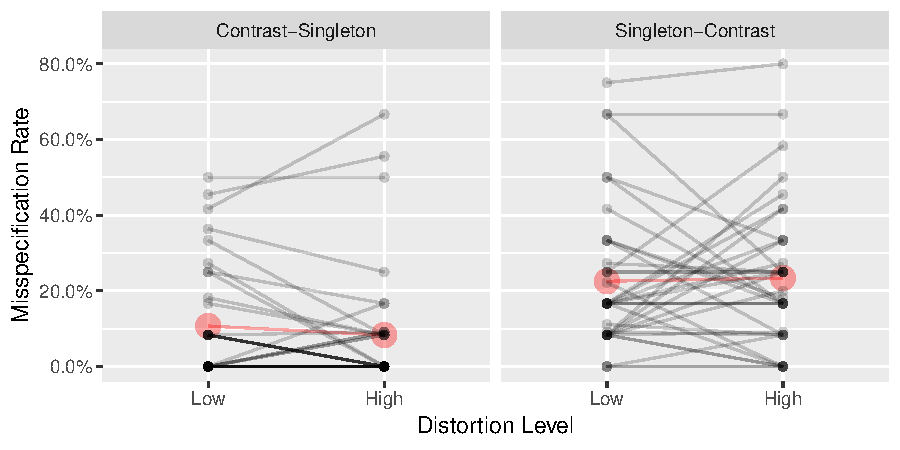
\includegraphics[width=.9\linewidth]{exp1/img/exp1-misrate-plot.pdf}
\caption{\label{fig:orgdb6176e}
Misspecification rate by Distortion Level and Shift Direction. Connected black points are individual participants and red points are grand means.}
\end{figure}

% latex table generated in R 3.3.3 by xtable 1.8-4 package
% Thu Feb 27 17:21:11 2020
\begin{table}[ht]
\centering
\caption{Distribution of utterance types across condition, Experiment 1.} 
\label{tbl:exp1-utt-dist}
\begin{tabular}{llrrrrrr}
  \hline
Shift Direction & Distortion & NO & PR & PO & AS & DE & AO \\ 
  \hline
Contrast-Singleton & Low & 89.4\% & 6.4\% & 1.7\% & 0.7\% & 1.9\% & 0.0\% \\ 
  Contrast-Singleton & High & 92.0\% & 3.9\% & 1.5\% & 0.0\% & 2.7\% & 0.0\% \\ 
  Singleton-Contrast & Low & 1.9\% & 58.4\% & 18.8\% & 14.3\% & 3.3\% & 3.3\% \\ 
  Singleton-Contrast & High & 1.7\% & 58.6\% & 17.5\% & 14.4\% & 4.1\% & 3.6\% \\ 
   \hline
\end{tabular}
\end{table}


Table~\ref{tbl:exp1-utt-dist} shows strong differences in the distribution of utterance types across the levels of \emph{Shift Direction}, but little evidence for any effect of \emph{Distortion}.  When speakers had entrained on modified nouns and were tested in a context requiring a bare noun, speakers only overspecified about
9.3\%
of the time overall.
Speakers were far more likely to misspecify references when they had entrained on bare nouns and the test context required a modifier. About
23.1\%
of the time speakers failed to include a modifer in the first instance (pre-nominally or post-nominally). Typically, if a modifier was included, it was included as a self-repair (``the W\ldots{} uh small W'').

For the inferential analysis of misspecification rate, we performed logistic regression using \texttt{glmer()}.  The logistic regression model converged with maximal random effects, but reported singularity in the variance-covariance matrix. Given doubt as to the interpretation of singular models \citep{bates-pmm}, we fit a second model in which we reduced the random effects structure until the singularity was removed. This second model included a random intercept and random slopes for \emph{Shift Direction} and the interaction term, but not for \emph{Distortion}. We report results from the second model.

There was little evidence to support the main prediction of a main effect of \emph{Distortion}. Misspecifications were observed on 
16.6\%
of trials in the \emph{Low Distortion} condition, compared to 
15.8\%
in the \emph{High Distortion} condition.
This difference was not significant (pre-registered one-tailed test),
\(\beta = 0.14\), \(SE = 0.16\), Wald \(z = 0.87\), \(p = 0.191\).
There was also little evidence for an interaction between \emph{Shift Direction} and \emph{Distortion}, 
\(\beta = -0.41\), \(SE = 0.37\), Wald \(z = -1.11\), \(p = 0.267\).
The effect of \emph{Shift Direction}, in contrast, was significant,
\(\beta = 1.47\), \(SE = 0.32\), Wald \(z = 4.53\), \(p < .001\).

\subsubsection*{Speech onset latency}
\label{sec:org6f1499e}

Our second main prediction concerned the differential speech onset latency for appropriately specified descriptions. Our prediction was that speakers would be less likely to shift from the entrained description to a more contextually appropriate description in the \emph{Low Distortion} condition than in the \emph{High Distortion} condition, due to a stronger retrieval of the entrained response.  For this analysis, in addition to the 51 trials excluded for reasons detailed above, a further 272 trials were excluded where speakers misspecified the target, and two more where the speech onset could not be determined.

\begin{figure}[htbp]
\centering
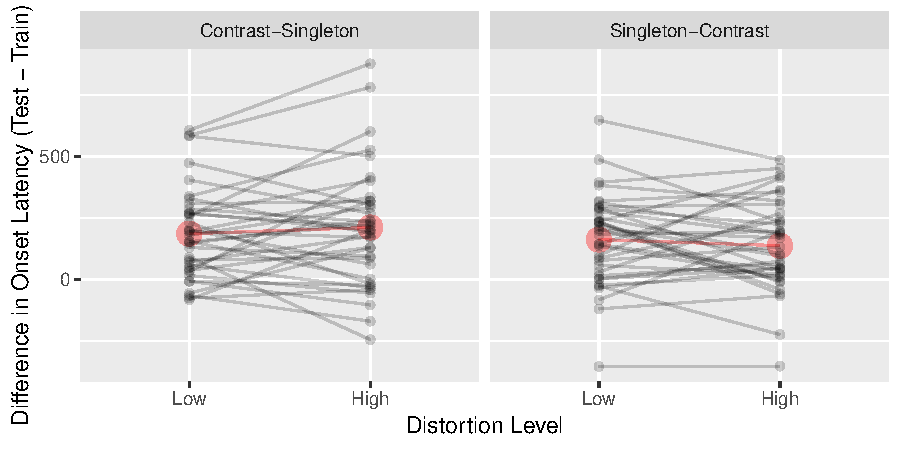
\includegraphics[width=.9\linewidth]{exp1/img/exp1-sol-plot.pdf}
\caption{\label{fig:org4f61e1d}
Change in speech onset latency from training to test by Shift Direction and Distortion Level. Positive values indicate higher latencies at test; connected black points are individual participants and red points are grand means.}
\end{figure}

The data are shown in Figure~\ref{fig:org4f61e1d}. Parameters were estimated using the \texttt{lmer()} function under maximum likelihood with identity link and Gaussian variance. The dependent variable was the speech latency for the test trial minus the speech latency for the final training trial for that sequence; in other words, the change in speech latency incurred by abandoning the entrained description. We tested against the null using a two-tailed test on the Wald \(z\) statistic with \(\alpha = .05\).  

We once again encountered singularity when fitting the maximal random-effects model, so we fit a second model with reduced random effects (the converging non-singular model had random intercepts and random slopes for \emph{Shift Direction}). Again, we report the results from the non-singular model.

The main prediction that speakers would encounter greater difficulty producing appropriately specified descriptions in the \emph{Low Distortion} condition was not supported: there was only a difference of 
5~ms
between the Low and High conditions, with means of 
\(M = 175\)~ms \((SD = 421)\) and
\(M = 180\)~ms \((SD = 444)\)
respectively, and a non-significant main effect of \emph{Distortion}, 
\(\beta = 0.63\), \(SE = 21.48\), Wald \(z = 0.03\), \(p = 0.977\).
There was also no significant main effect of \emph{Shift Direction}, 
\(\beta = -53.17\), \(SE = 47.94\), Wald \(z = -1.11\), \(p = 0.267\). 
Finally, the interaction was also not significant,
\(\beta = 57.24\), \(SE = 43.13\), Wald \(z = 1.33\), \(p = 0.184\).

\subsubsection*{Eye gaze}
\label{sec:org16ac083}

\begin{figure}[htbp]
\centering
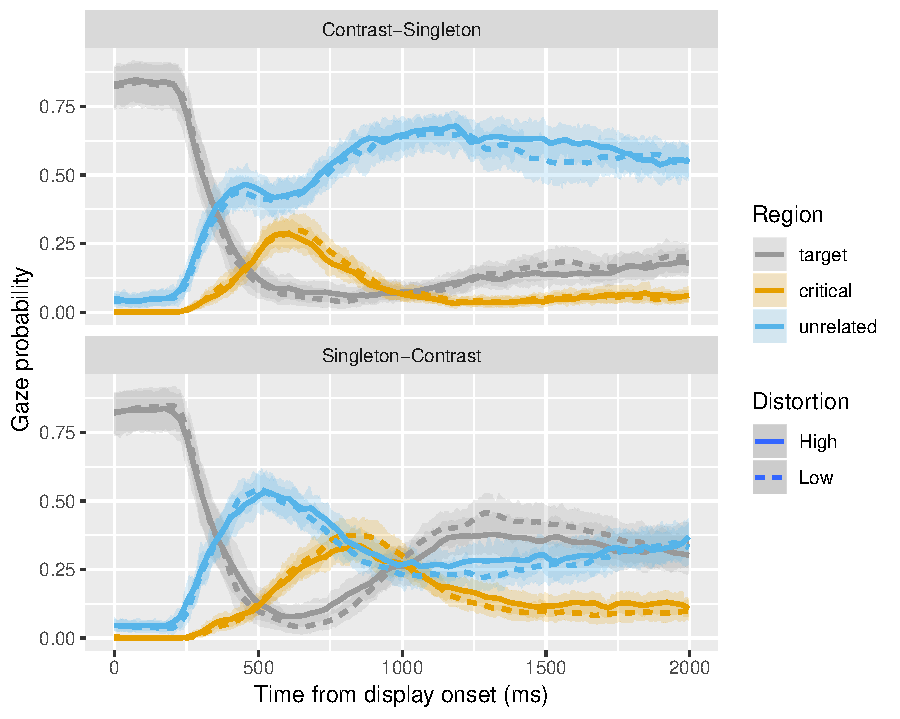
\includegraphics[width=.9\linewidth]{exp1/img/exp1-probplot.pdf}
\caption{\label{fig:org02353c6}
Gaze probability by Shift Direction and Distortion. The critical image was a competitor in the Singleton-Contrast condition and a foil in the Contrast-Singleton condition. The shaded region around each line represents the 95\% confidence interval obtained by bootstrapping subjects.}
\end{figure}

The modest rate of misspecification in the experiment indicates reliance on memory, but we found no clear evidence for the main prediction of stronger retrieval of entrained descriptions in the \emph{Low Distortion} condition. This result is ambiguous: it could be taken as support for the idea that speech content is not strongly influenced by ordinary memory processes, but only if the manipulation of layout was successful in inducing stronger memory associations in the \emph{Low Distortion} condition.  

To verify this, we plotted the probability of gazing at various types of images over time (Figure~\ref{fig:org02353c6}).  There is some suggestion that the memory manipulation was effective in the predicted direction, but the effect appears small. The figure indicates that speakers typically started the trial already fixated on the pre-cued target image and began looking away about 250~ms after display onset. Speakers appear to look away from the target and toward the critical image (competitor or foil) slightly more rapidly in the \emph{Low Distortion} condition. Although the pattern is consistent with stronger memory effects in the \emph{Low Distortion} condition, the size of the effect is not such to fully rule out the possibility that the memory manipulation was too weak.

We also carried out our pre-registered test of a difference in the rate of non-target fixations prior to speech onset for appropriately-specified descriptions. We predicted a higher fixation rate for the \emph{Low Distortion} condition. We fit a generalized linear mixed effects model to the count data with a log link and Poisson variance function. The model included a by-subjects random intercept and a random slope for the effect of \emph{Distortion}. The covariance matrix for random effects was singular, so we dropped the random slope and re-fit the model. 

No statistically significant difference was detected (two-tailed) between the mean fixation rates of 
1.45 (SD = 0.63) for the \emph{Low Distortion} condition, and
1.44 (SD = 0.62) for the \emph{High Distortion} condition,
\(\beta = 0.01\), \(SE = 0.04\), Wald \(z = 0.15\), \(p = 0.882\).

\section*{Experiment 2}
\label{sec:orgfaab9e3}
Although the high misspecification rate in Experiment~1 unequivocally demonstrates the involvement of memory processes, the non-verbal eye gaze measurements suggest that the main manipulation may have been too weak. Experiment~2 included several improvements to increase training-test similarity and strengthen the memory associations with the target descriptions.

\begin{figure}[htbp]
\centering
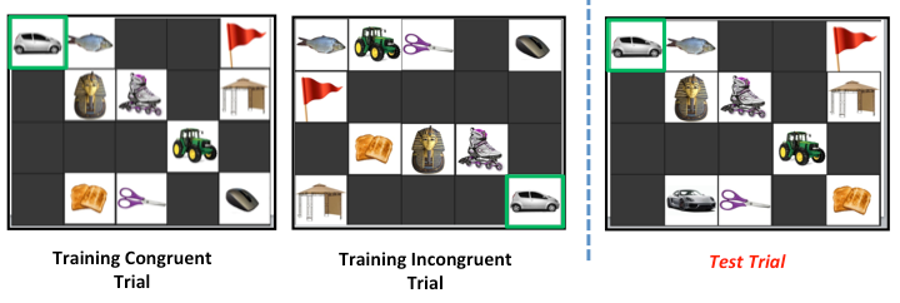
\includegraphics[width=.9\linewidth]{figs/Exp2_overview.png}
\caption{\label{fig:orgf38b6ea}
Example training and test displays, Experiment 2. The target was indicated to the speaker by a green square surrounding the image.}
\end{figure}

It is possible that memory effects in Experiment~1 were obscured by the high similarity among memory representations across stimulus items. All of the target items were letters of the alphabet, and the only type of modification ever required was a size modification (e.g., ``the small W''). This would have created high overlap among memory representations that could have led to interference during retrieval. We sought to minimize interference using variety of everyday objects as targets and competitors in Experiment~2 (Figure~\ref{fig:orgf38b6ea}), similar to the type of stimuli used in \cite{GannBarr2014}. For each pair, the target was always a very typical member of the category (moreso than the competitor), such that when described in a context by itself there would be a strong tendency to use a basic level term (e.g., the candle, the apple, the car) \citep{roschetal76}. Competitors were chosen so as to elicit target modifiers that would be very unlikely to occur in the absence of the target. For the candle example, the the competitor was a highly similar half-melted candle, such that a typical description of the target would be ``the unmelted candle.''  We chose foil objects that were visually similar to the competitor but from a different category of object. For a full list of target-competitor-foil triplets, see the supplementary materials in the data repository.

The above manipulation also addresses an additional weakness of Experiment~1, which was the high rate of data loss due to speakers who opted for a strategy of always including a size modifier, whether or not it was needed. In this experiment, speakers would need to focus on different dimensions for each category of object, which was intended to discourage this strategy and reduce data loss.

A second way we sought to strengthen memory effects was by removing pre-cuing of the target location. In the previous experiment, before the target or any other images appeared, speakers were directed toward the target's location. Since the location itself might operate as a memory cue, retrieval processes may have already begun prior to display onset, making their effects less detectable when they were measured at a later point.  To remedy this, in the current experiment, the highlight indicating the target location occurred simultaneously with display onset.

Finally, instead of creating low and high distortions of a single spatial arrangement prototype, we simply manipulated whether the arrangement at test was identical to the training arrangement (\emph{Congruent} condition), or a different random arrangement (\emph{Incongruent} condition), forming the factor of \emph{Congruency} (Figure~\ref{fig:orgf38b6ea}). Note that for the \emph{Incongruent} displays, the target location remained fixed over training and test displays, while the locations of all other images (including the competitor/foil) were randomized.

\subsection*{Method}
\label{sec:org7579b6d}

The method of Experiment~2 was similar to Experiment~1, and so we only describe the differences. A link to the pre-registration for this experiment can be found in the OSF repository.

\subsubsection*{Participants}
\label{sec:org44d7cf7}

We collected data from a a total of 37 University of Glasgow students (24~women and 13~men), with data from one participant excluded due to overdescribing in more than 50\% of the last training trials before the corresponding test trial. All participants were paid £6 or received course credit.

\subsubsection*{Design}
\label{sec:org24a78a5}

There were two factors in the design, \emph{Congruency} (\emph{Congruent} versus \emph{Incongruent}) and \emph{Shift Direction} (\emph{Singleton-Contrast} and \emph{Contrast-Singleton}), forming a full-factorial 2x2 within-participant design.  Both factors were also manipulated within each stimulus set.

\subsubsection*{Materials}
\label{sec:orgcb0d8ce}

Each display consisted of a five-by-four grid containing various types of everyday objects (see Figure~\ref{fig:orgf38b6ea}). The experiment contained 48 ``sequences'' of trials, each consisting of a number of training trials followed by a single test trial (with each sequence being defined as the collection of training and test trials all associated with a single target/competitor/foil triplet). Each triplet appeared an equal number of times in all four conditions of the 2x2 design, counterbalanced across participants using stimulus lists.

For each sequence, the number of training trials was randomly selected, with a range from 6 to 9. Given these parameters, each experimental session could have contained between 336 (7 x 48) and 480 (10 x 48) trials. For each stimulus set, 7 to 10 additional images unrelated to the target were randomly chosen from a database of stimulus images. Images were re-used across trials within a sequence, but not across different stimulus sets. The displays were checked manually by two lab assistants to ensure that the unrelated items were sufficiently dissimilar to the target so as not to influence descriptions of the target.

Target and competitor items were normed beforehand by 68 Native English speaking volunteers using the web-based survey platform SurveyMonkey. A number of items were updated or replaced based on our norming feedback. Four entirely new stimuli pairs were added to our original list (for a complete list of the Target and Competitor objects used please see the supplementary information provided in the OSF repository).

\subsubsection*{Apparatus}
\label{sec:org9763722}

The apparatus was identical to Experiment~1, with the exception that the eyetracking sampling rate for all participants was set to 250~Hz.

\subsubsection*{Procedure}
\label{sec:orgbb4f906}

The procedure was identical to the previous experiment, with the exception that on each trial, the cue for the target location appeared simultaneously with the rest of the display.  Additionally, although speakers and listeners had different arrangements of each set of images within the grid, the listener's arrangement was held constant within each sequence to facilitate easier identification of the target. Our rationale was that with predictable target locations, listeners would be faster to identify targets during training, which might lead the speaker to entrain more strongly on the referential precedent.

\subsubsection*{Data Analysis}
\label{sec:org580254e}

The measurements and predictions were identical to Experiment~1, with the difference that all mixed-effects models also included by-item random intercepts and slopes, since items (sets of target/competitor/foil/unrelated images) repeated across participants and were likely to induce different patterns of modification.

Occasionally a speaker would use a single subordinate-level term to distinguish the target from the competitor (e.g., ``notes'' instead of ``paper money'' to distinguish a stack of notes from a pile of coins). In these instances, we coded the speech as category \emph{PR}. Cases where speakers provided disambiguating information after as well as before the head noun (``the woolen gloves that are red''), were coded as \emph{PR}, as long as the information before the head noun seemed sufficient to disambiguate the target from the competitor. Thus, the choice of \emph{PR} versus \emph{PO} captures whether any adaptations took place up to (and including) the head noun, or somewhere after (\emph{PO}).

Unlike Experiment~1, we only coded speech onset times for appropriately-specified descriptions. Another difference was that we also established exclusion criteria for items (stimulus sets). We considered the last training trial for each participant on each item on which the critical object was a foil, and removed items where speakers used a modifier that would have distinguished the target from the (absent) competitor. Any items where the rate of modifier use was greater than 50\% was removed.

\subsection*{Results and Discussion}
\label{sec:orgb624554}

Of the 1728 test trial observations we recorded, we removed 252 from seven stimulus items that met our exclusion criterion (see above), and an additional 176 observations where either speakers had used a modifier in the last training trial where it was not appropriate (143), or the response could not be identified from the sound recording (33). This left 1300 trials remaining for the analyses below.

\subsubsection*{Misspecification rate}
\label{sec:orgfe57d46}

\begin{figure}[htbp]
\centering
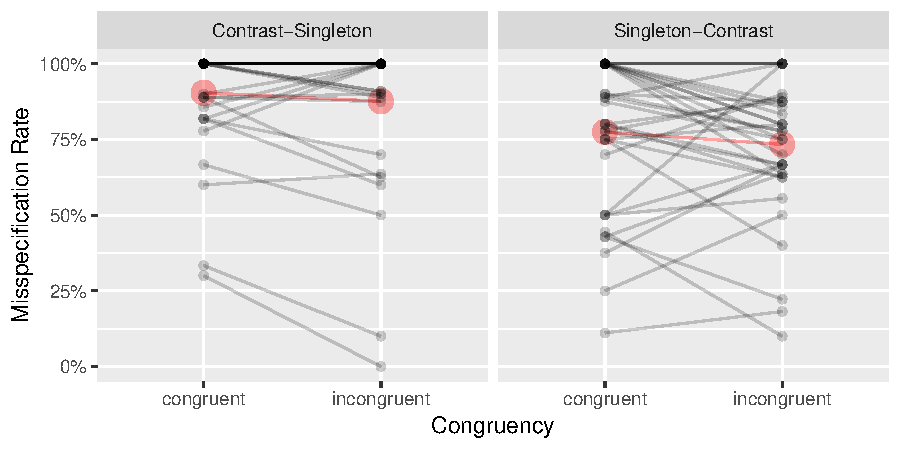
\includegraphics[width=.9\linewidth]{exp2/img/exp2-misrate-plot.pdf}
\caption{\label{fig:org3321719}
Misspecification rate by Congruency and Shift Direction. Connected black points are individual participants and red points are grand means.}
\end{figure}

% latex table generated in R 3.3.3 by xtable 1.8-4 package
% Thu Feb 27 17:21:26 2020
\begin{table}[ht]
\centering
\caption{Distribution of utterance types across conditions.} 
\label{tbl:exp2-utt-dist}
\begin{tabular}{llrrrrrr}
  \hline
Shift Direction & Congruency & PR & AO & AS & PO & NO & DE \\ 
  \hline
Contrast-Singleton & Congruent & 76.4\% & 0.0\% & 0.3\% & 12.1\% & 9.5\% & 1.7\% \\ 
  Contrast-Singleton & Incongruent & 75.4\% & 0.0\% & 0.3\% & 10.7\% & 12.4\% & 1.2\% \\ 
  Singleton-Contrast & Congruent & 12.4\% & 53.0\% & 22.5\% & 8.4\% & 3.4\% & 0.3\% \\ 
  Singleton-Contrast & Incongruent & 21.4\% & 47.6\% & 21.1\% & 6.1\% & 2.7\% & 1.0\% \\ 
   \hline
\end{tabular}
\end{table}

Table~\ref{tbl:exp2-utt-dist} shows strong differences in the distribution of utterance types across the levels of \emph{Shift Direction}, but little evidence for any effect of \emph{Congruency}.  When speakers entrained on modified nouns, overspecification at test occurred in about
89.1\%  
of cases. When they entrained on bare nouns, 
74.5\%
of cases failed to include a modifer in the first instance; typically, if a modifier was included, it was included as a self-repair.

For the misspecification rate analysis, we performed logistic regression using \texttt{glmer()}.  The logistic regression model of misspecification rate converged with maximal random effects, but reported singularity in the variance-covariance matrices. We fit a second model in which we reduced the random effects structure until the singularity was removed. The model that converged included by-subject and by-item random intercepts; by-subject random slopes for \emph{Shift Direction}, \emph{Congruency}, and their interaction; and by-item random slopes for \emph{Shift Direction} and \emph{Congruency} but not for the interaction. All covariance parameters were constrained to zero.  We report the results from the second model.

There was some evidence for the main prediction: misspecifications were observed on 
84.5\%
of trials in the \emph{Congruent} condition, compared to 
80.1\%
in the \emph{Incongruent} condition, a significant main effect of \emph{Congruency}, (pre-registered one-tailed test), 
\(\beta = 0.42\), \(SE = 0.22\), Wald \(z = 1.88\), \(p = 0.030\).
There was little evidence for an interaction between \emph{Shift Direction} and \emph{Congruency}, 
\(\beta = -0.10\), \(SE = 0.41\), Wald \(z = -0.25\), \(p = 0.806\).
The effect of \emph{Shift Direction}, in contrast, was significant,
\(\beta = -1.71\), \(SE = 0.38\), Wald \(z = -4.56\), \(p < .001\).

\subsubsection*{Speech onset latency}
\label{sec:org756e0a7}

As in the previous experiment, the prediction was that speakers would have more difficulty shifting to an appropriately specified test description when memory associations were stronger (i.e., in the \emph{Congruent} condition). 
The means in the \emph{Congruent} and \emph{Incongruent} conditions were inconsistent with this prediction,
\(M = 2277\)~ms \((SD = 975)\)
and 
\(M = 2481\)~ms \((SD = 981)\)
respectively. 
However, the very high rate of misspecification in the current experiment
(82.3\%)
left very few appropriately-specified observations for analysis 
(only 230).
Given the very small number of remaining observations, we opted to forgo any further statistical analysis. Because we only had onset data for a small minority of observations, we also did not pursue our pre-registered analysis of the rate of pre-onset fixations across congruency conditions.

\subsubsection*{Eye gaze}
\label{sec:orgb3a98ae}

\begin{figure}[htbp]
\centering
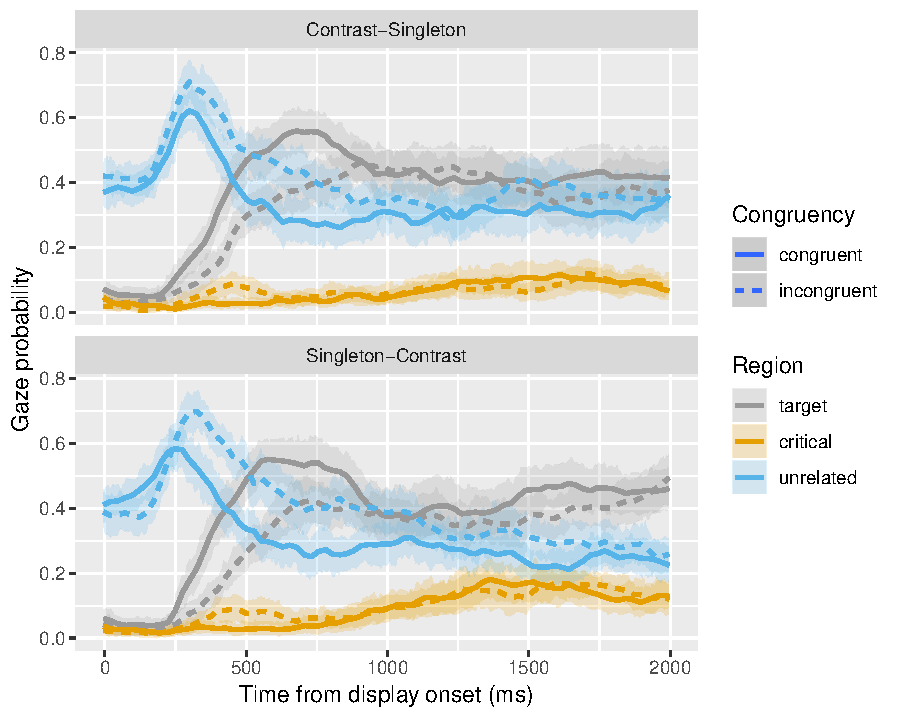
\includegraphics[width=.9\linewidth]{exp2/img/exp2-probplot.pdf}
\caption{\label{fig:orge60f1dd}
Gaze probability by Shift Direction and Congruency. The critical image was a competitor in the Singleton-Contrast condition and a foil in the Contrast-Singleton condition.}
\end{figure}

In contrast to Experiment~1, a plot of the probability of eye gaze on the various regions (Figure~\ref{fig:orge60f1dd}) indicates unequivocal memory effects: when the display arrangement was congruent at test, speakers looked away from the target and toward the critical object much more rapidly.

Unlike the previous experiment, the main prediction did receive some statistical support: speakers relied on remembered descriptions significantly more often when the arrangement of the test display was more similar to the arrangement at training.  However, the effect of similarity was small, corresponding to about a 
4.5\%
difference that only barely reached significance. In contrast, the differences in eye movements were quite strong: for instance, the rate of fixating on the target 500~ms after onset was about 50\% in the \emph{Incongruent} condition versus 30\% in the \emph{Congruent} condition. So although perceptual aspects of the conversational situation are clearly stored and affect processing, these aspects may only have very weak effects on speech content.

One notable difference from Experiment~1 was the very high overall misspecificaton rate, which was about 
82.3\%, compared to about 
16.2\% 
in Experiment~1.  What might account for this difference?  This might be attributable to semantic/pragmatic differences between size modifiers and other types of modifiers. Perhaps because size modifiers have more relational semantics than other types of modifiers \citep{GrodnerSedivy2011}, they are used in a more context-specific manner. Another possibility is that the constant use of size modification in Experiment~1 led speakers to pay more attention overall to the presence or absence of a size contrast in any given display.

\section*{Experiment 3}
\label{sec:org4c03956}

In Experiments~1 and~2, we used spatial arrangement as a memory cue. While spatial cues allow convenient measurement of implicit aspects of memory processes through eyetracking, they have the disadvantage of potentially low ecological relevance for communication. Although the eye movement data showed that speakers did indeed store information about spatial configuration, spatial information is not something that speakers need to regularly attend to for their references to succeed. The perceptual information associated with conversational partners provides a far more important and ecologically relevant set of cues.

When language users interact, particularly in a face-to-face setting, it would seem likely that they would develop links between the content of the dialogue and perceptual features of their interactions, such as how their interlocutors look and sound. The ordinary memory view assumes that these perceptual features can drive a resonance process that makes relevant information from past conversations readily accessible \citep{hortongerrig05}. We designed Experiment~3 around this key assumption. 

\begin{figure}[htbp]
\centering
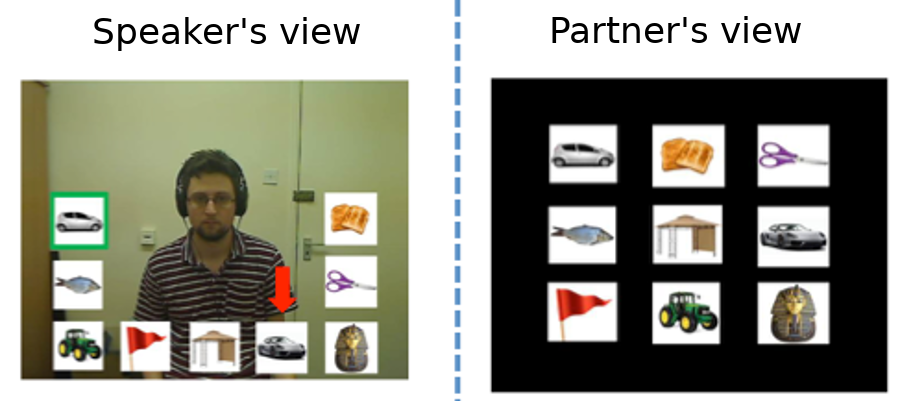
\includegraphics[width=.9\linewidth]{figs/Exp3_C-S.png}
\caption{\label{fig:orgefe8906}
Example displays for the speaker and the confederate partner, Experiment 3. (Note that the red arrow, which indicates the location of the competitor, is included for expository convenience, but did not appear on the speaker's display.)}
\end{figure}

Sighted language users in Western cultures generally look at their addressees while communicating. As a result, the perceptual experience of seeing one's partner is confounded with the speaker's mental representation of that person's conversational role as an addressee. For the purpose of our study, it was necessary to deconfound these two streams of information to be able to measure memory effects independently from effects about the speaker's beliefs their common ground with the addressee.  We did this by having speakers communicate with two different partners over independent video and audio links. Both of the partners were together, but in a separate room from the speaker.  The two partners (who were experimenters) alternated in their role as addressee.  The video link showed one of the two partners at a time. We manipulated which partner appeared on the speaker's screen independently from which partner had access to the audio link relaying the speaker's live speech. This setup makes it possible for speakers to be looking at one partner who cannot hear them while addressing another, unseen partner.

During training phases, speakers developed memory associations between targets and expressions while addressing and viewing one of two partners. Both partners wore headphones; during training, the on-screen partner could hear and respond to descriptions via audio link, while the off-screen partner wore a blindfold and heard masking noise to limit their access to the exchange.  The images that the speaker conversed about appeared superimposed over the image of the partner (see Figure~\ref{fig:orgefe8906}). The objects depicted in the images were similar to the ones we used in Experiment~2 and, as in that experiment, speakers also entrained on either modified or unmodified descriptions. Note that during training, the visible partner and the addressee were one and the same.

\begin{figure}[htbp]
\centering
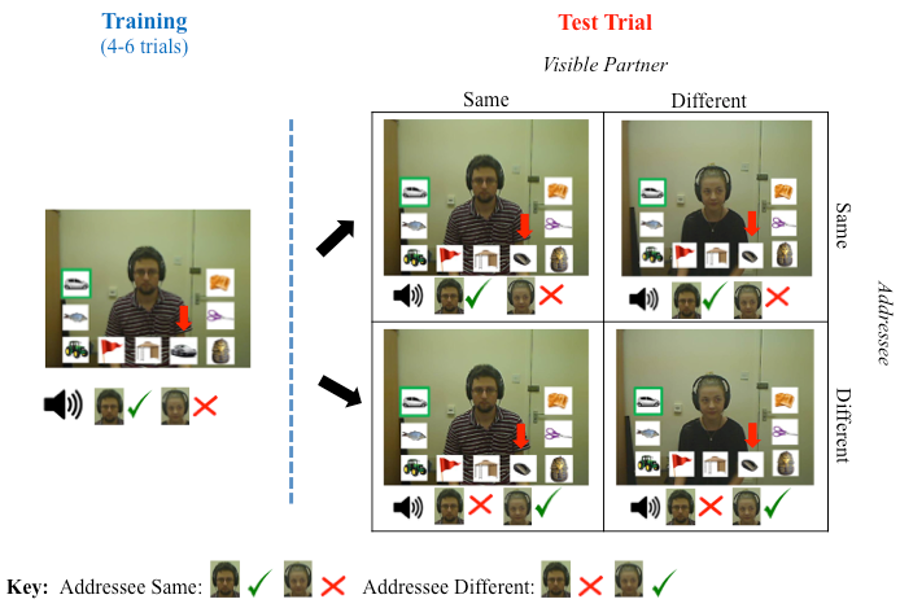
\includegraphics[width=.9\linewidth]{figs/Exp3_overview.png}
\caption{\label{fig:orgb408182}
Design of Experiment 3, showing one training and one test trial for an example item in the Contrast-Singleton condition. The four versions of the test trial correspond to all four conditions obtained by factorially combining Visible Partner and Addressee. The red arrow indicates the competitor/foil object for expository purposes, and was not shown on the speaker's display.  The loudspeaker icon indicates which partner was the addressee (i.e., could hear the speech) on that trial in that condition.}
\end{figure}

As in the previous experiment, test trials differed from training trials in the identity of a critical object: in the \emph{Singleton-Contrast} condition, the foil from training became a competitor at test (potentially inducing underspecification of the target), while in the \emph{Contrast-Singleton} condition, the competitor at training became a foil at test (potentially inducing overspecification of the target). We also independently manipulated the congruence of the test situation with the training situation along two separate dimensions: \emph{Addressee} (same or different) and \emph{Visible Partner} (same or different; see Figure~\ref{fig:orgb408182}). The critical question was whether speakers would be more likely to misspecify referents at test when the visible partner was the same as the one they had seen (and spoken to) during training, compared to when it was the partner they had not spoken to.  If partners serve as memory cues, speakers should be more likely to misspecify referents at test when they are looking at the partner they spoke to during training (regardless of whether they are currently addressing this partner). To maximize power, we pre-registered a one-tailed test of this prediction (greater misspecification in the \emph{Visible Partner: Same} condition).  Additionally, the inclusion of the \emph{Addressee} factor makes it possible to test the extent to which misspecified descriptions are the result of speakers using common ground---that is, of them preferring to continue using an established precedent because it is part of their common ground with the addressee \citep{brennanclark96}. Under this view, speakers should misspecify more often when they are speaking to the same addressee, regardless of which partner is visible.

Dissociating visibility from participant roles required a complex setup, raising the possibility of speakers becoming confused about who could and could not hear them at any given point in time. We took several steps to ensure speakers were clear about what was going on. First, the identity of the visible partner and addressee remained fixed over a block of trials, rather than changing with each trial. Before any such block began, speakers were presented with a notification of who should be the addressee for that block. Speakers were made responsible for selecting that person as the addressee by manipulating a crossfader knob on an audio mixer. Thus, speakers had to attend to and act on the information about the addressee's identity. Second, during a warm-up phase of the experiment, speakers were given the opportunity to play the role of both addressee and non-addressee while one of the listeners took the role of the speaker. This made it clear to participants that the non-addressed partner would lack knowledge of the established referential precedents. 

\begin{figure}[htbp]
\centering

\includegraphics[width=.9\linewidth]{figs/Exp3_unconv.png}
\caption{\label{fig:org5c2f8e4}
Unconventional targets used in Experiment 3.}
\end{figure}

Finally, we included an additional set of unconventional targets (Figure~\ref{fig:org5c2f8e4}) which served primarily as a check on whether speakers were attending to the identity of the addressee. These unconventional targets were abstract shapes that could only be identified using structural descriptions. We included these because we have previously found that these materials elicited strong effects of common ground \citep{GannBarr2014}. Speakers gradually shorten their descriptions of unconventional objects when they refer to them repeatedly with the same addressee \citep{clarkwilkesgibbs86}. Most importantly, when they describe old referents to new addressees who lack knowledge of the previous descriptions, they tend to lengthen their descriptions. To a large extent, this lengthening appears to be the result of incrementally elaborating upon the informationally-reduced descriptions arrived at with the old partner, rather than planning entirely new descriptions \citep{GannBarr2014}. Given this prior research, we expected speakers to produce longer descriptions for these targets when speaking to new addressees.

\subsection*{Method}
\label{sec:orgc03112f}

A link to the pre-registration for this experiment can be found in the OSF repository.

\subsubsection*{Participants}
\label{sec:orgddb5ea9}

The final dataset included data from a total of 40 University of Glasgow students (31~women and 9~men), all of whom identified themselves as native English speakers. Data from one additional participant was replaced due to continuously failing to provide informationally adequate descriptions during training (54.2\% misspecifications on the last training trial before test). All participants were paid £6 or received course credit.

\subsubsection*{Design}
\label{sec:org322b945}

The study had a 2x2x2 design, with factors \emph{Shift Direction} (\emph{Singleton-Contrast}, \emph{Contrast-Singleton}), \emph{Addressee} (\emph{Same}, \emph{Different}), and \emph{Visible Partner} (\emph{Same}, \emph{Different}). The levels of all factors were administered within participants and within stimulus items.

\subsubsection*{Experimental setup and task}
\label{sec:orgdbbfd2c}

As in the previous experiments, speakers were to describe the target object on each trial so that an addressee could identify it. The addressee could be one of two partners (a male or female experimenter), but only one of them could actually hear the description. For the speaker, each display consisted of nine images of various objects displayed around the webcam image of the visible partner (see Figure~\ref{fig:orgefe8906}). Only one of the two partners was on-screen at a given time.  The partners saw only a 3x3 grid of objects, and indicated their choice by pressing a key on a number pad.

There were 48 main sets of stimuli, presented over 12 blocks of trials, with each block further subdivided into training and test phases. Each block was in one of the four conditions obtained by factorially combining the levels of \emph{Addressee} (\emph{Same}, \emph{Different}) and \emph{Visible Partner} (\emph{Same}, \emph{Different}), with the presentation order of the blocks determined randomly for each participant.  Two of the four stimulus sets in each block appeared in the \emph{Singleton-Contrast} condition, while the other two appeared in the \emph{Contrast-Singleton} condition.  The assignment of stimulus sets to condition was counterbalanced using eight presentation lists, with five participants randomly assigned to each list, such that each set appeared in all eight conditions of the design across participants.

\subsubsection*{Apparatus}
\label{sec:orga64765b}

The experimental stimuli were presented on a 19'' LCD Dell desktop computer monitor (4:3 aspect ratio, resolution 1024 x 768 pixels). A microphone was placed above the participant's computer monitor to record their descriptions of the target object for each trial. Speakers controlled the crossfader on a Numark two input stereo mixer with a crossfading slider. One input had the white noise coming in on the left channel and live audio from the microphone on the right channel; the other input had the opposite configuration.  The left output channel was split and fed from the mixer to one set of headphones, while the right output channel was split and fed to the other set of headphones.  With this configuration, by sliding the crossfader all the way to the left, one participant would hear speech and the other would hear the white noise; sliding it all the way to the right would create the opposite situation.  The two ends of the crossfader were colored so as to identify which partner would be the addressee by sliding the knob in that direction.

Video from the room with the two partners was recorded using a Logitech Pro 9000 webcam and transmitted to the speaker's display.

\subsubsection*{Materials}
\label{sec:org6854103}

We re-used the stimuli from Experiment~2, except we replaced nine of the target/competitor/foil triplets with new sets, including the seven sets that were excluded from Experiment~2 due to high rates of misspecification during training.  See the online repository for a list of the 48 target and competitor pairs.  A third of the targets were randomly assigned to four training repetitions, a third to five training repetitions, and a third to six, forming a total of 240 training trials across all blocks for each session, and 48 test trials.

Each of the twelve blocks included two additional sets of stimuli. One of these sets consisted of filler items that we included so that a change from training to test (with a possible change of visible partner and/or addressee) did not always require a change in the description of the targets (i.e., there was no substitution of the foil/competitor from training to test). There were twelve of these sets, one for each block, half of which were constructed so that reference to the target required a modifier, and the other half so that it required no modification.  The targets were repeated three times during training and once at test, forming a total of 48 trials for each session.

The other set of stimuli included in each block consisted of the unconventional targets (as described above). In each block, one unconventional target was repeated three times during training, and once at test, forming 48 additional trials for each session.

In sum, there were 384 trials in total for each experimental session: 240 training trials (4 items repeated 4-6 times in each block), 48 test trials (4 items per block), 48 fillers with targets modeled after the main stimulus items (1 item per block repeated four times), and 48 items with unconventional targets (1 item per block repeated four times).

\subsubsection*{Procedure}
\label{sec:orgb078f1b}

Upon arrival each participant was given an instruction sheet detailing the task and their role during the experiment (see OSF repository for details). The two partners were set up in an adjoining room to the speaker and faced a single computer monitor. 

The partners were seated in rolling chairs, which allowed them to easily slide in front of or away from the camera, as required. The floor of the lab room was marked with tape to indicate where chairs needed to be positioned to be on or off camera. To minimize confusion for the speaker, each partner wore a colored tag that corresponded to the color of a sticker placed at each end of the crossfading slider. 

Before the experiment began participants took part in a practice session that consisted of twelve training trials and four test trials.  This enabled the participant to familiarise themselves with their role as speaker, as well as to experience the task from the perspective of the partner. In this manner, the participant was made aware that the partners saw the images in an entirely different spatial arrangement (Figure~\ref{fig:orgefe8906}) and that only one partner at a time would be able to hear the descriptions. After practice ended, the main part of the experiment began.

On each trial, audio recording began simultaneously with the presentation of the display. The target object in each display was highlighted for the speaker by a green square. The trial ended when the addressee selected an object on the number pad. The speaker received no feedback regarding which picture the addressee selected. If the speaker failed to provide sufficient information to identify the target, the addressee would ask for clarification. Any such clarification exchanges appeared in the audio recording for the trial and were noted during later transcription.

Before each block of training trials, an on-screen notice informed the speaker which partner would appear on-screen and which partner would be the addressee. In the notice, the partners were identified by both color (the yellow and the orange partner) and first name. Partners wore different color name tags that matched the color of two stickers placed on either end of the crossfader on the audio mixer. 

The on-screen notice before each training phase also indicated that the off-screen partner was to put on the blindfold. Based on the notice, the speaker slid the crossfader to the appropriate color to select the next addressee.  Each of the two partners served as the training phase addressee for six of the twelve blocks.  The partner who was not selected as addressee during training was always off-screen wearing a blindfold, and could only hear white noise through their headphones.

Just prior to the test phase another on-screen notice appeared indicating that the blindfold was to be removed, and designated the identity of the on-screen partner as well as the addressee. Again, the participant was responsible for sliding the crossfader to the appropriate color. So that the delay between training and test would not be confounded with condition, the notice appeared for a minimum of eighteen seconds before advancing to the next phase, which provided more than sufficient time for the partners to move into position and for the speaker to select the specified addressee.

\subsubsection*{Data Analysis}
\label{sec:orgc2822ca}

We transcribed and coded each speaker's spoken responses as described in Experiment~2. Each speaker had 98 trials for coding/transcription: the 48 test trials, and the final training trial for each stimulus item prior to the test trial. As with the previous experiments, the training trials were coded to verify that speakers were not already misspecifying the referent during training. We also transcribed each speaker's description of the twelve unconventional targets at test, and counted the number of words used in the description.

The misspecification variable was analyzed using linear mixed-effects regression, estimated with the \texttt{glmer()} function from \texttt{lme4}, with a logit link function and binomial variance. For the random effects structure, we included by-subject and by-item intercepts and also sought to include by-subject and by-item random slopes for all main effects and interactions.

Word count for unconventional targets was analyzed using linear mixed-effects regression, estimated with \texttt{glmer()} with a log link function and Poisson variance. The maximal model structure we sought to fit included by-subject and by-item random slopes for \emph{Visible Partner}, \emph{Addressee}, and their interaction.

\subsection*{Results and Discussion}
\label{sec:org509ba9c}
We applied the same exclusion criteria for participants and stimuli in Experiment 3 as we did in Experiment~2. Based on these criteria one participant was replaced (as noted in \hyperref[sec:orgdb5993b]{Participants}) and two of the 48 stimulus sets were removed prior to analysis, leaving 1840 total trials.  Of these, an additional 131 were removed, 128 of which because the speaker did not appropriately specify the target on the final training trial, and three because the speech could not be determined due to poor recording quality.

\subsubsection*{Misspecification rate}
\label{sec:org2545054}

\begin{figure}[htbp]
\centering
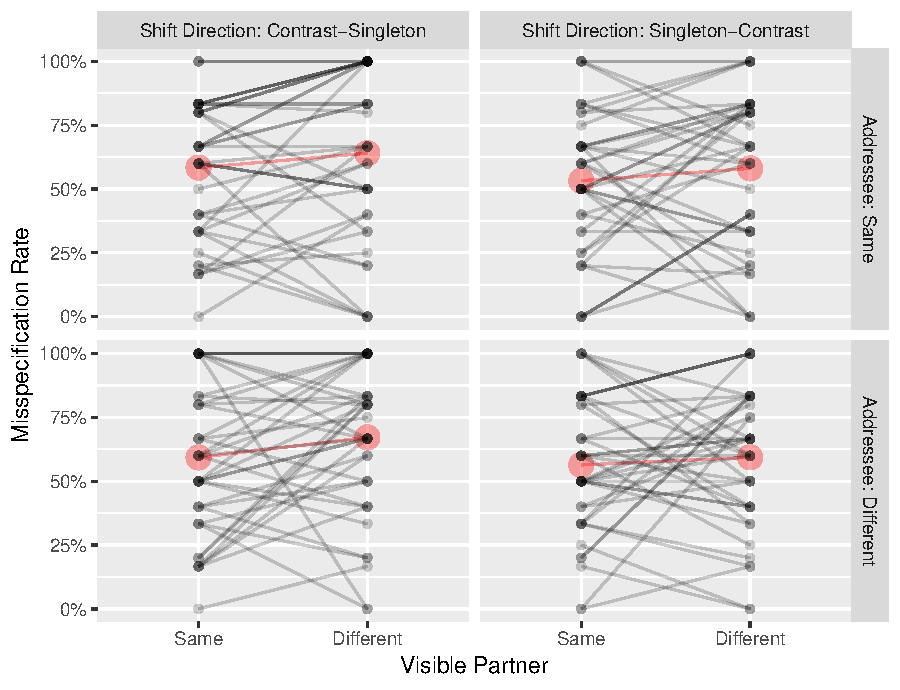
\includegraphics[width=.9\linewidth]{exp3/img/exp3-misrate-plot.pdf}
\caption{\label{fig:org29bbe29}
Misspecification rate by Visible Partner, Addressee, and Shift Direction. Connected black points are individual participants and red points are grand means.}
\end{figure}

% latex table generated in R 3.3.3 by xtable 1.8-4 package
% Thu Feb 27 17:21:38 2020
\begin{table}[ht]
\centering
\caption{Distribution of utterance types across Visible Partner and Addressee, Contrast-Singleton condition, Experiment 3.} 
\label{tbl:exp3-utt-dist}
\begin{tabular}{llrrrrrr}
  \hline
Visible Partner & Addressee & PR & NO & AO & PO & AS & DE \\ 
  \hline
Same & Same & 48.9\% & 41.2\% & 0.0\% & 9.0\% & 0.9\% & 0.0\% \\ 
  Same & Different & 45.5\% & 41.4\% & 0.0\% & 8.6\% & 1.4\% & 3.2\% \\ 
  Different & Same & 50.9\% & 34.1\% & 0.0\% & 11.4\% & 0.9\% & 2.7\% \\ 
  Different & Different & 51.4\% & 33.2\% & 0.0\% & 13.6\% & 0.0\% & 1.8\% \\ 
   \hline
\end{tabular}
\end{table}

% latex table generated in R 3.3.3 by xtable 1.8-4 package
% Thu Feb 27 17:21:39 2020
\begin{table}[ht]
\centering
\caption{Distribution of utterance types across Visible Partner and Addressee, Singleton-Contrast condition, Experiment 3.} 
\label{tbl:exp3-utt-dist}
\begin{tabular}{llrrrrrr}
  \hline
Visible Partner & Addressee & PR & NO & AO & PO & AS & DE \\ 
  \hline
Same & Same & 28.2\% & 2.0\% & 32.2\% & 15.8\% & 21.8\% & 0.0\% \\ 
  Same & Different & 23.0\% & 3.3\% & 33.0\% & 19.6\% & 20.6\% & 0.5\% \\ 
  Different & Same & 22.5\% & 2.5\% & 39.5\% & 17.5\% & 18.0\% & 0.0\% \\ 
  Different & Different & 23.2\% & 2.4\% & 38.4\% & 17.5\% & 18.5\% & 0.0\% \\ 
   \hline
\end{tabular}
\end{table}

The logistic regression model of misspecification rate did not converge with maximal random effects. We fit a second model in which we reduced the random effects structure until convergence was reached and no singularity message was encountered. The reduced model contained by-subject random intercepts, by-subject random slopes for \emph{Visible Partner}, the \emph{Visible Partner-by-Addressee} interaction, and the three way interaction, with covariances constrained to zero; by-item random intercepts, by-item random slopes for \emph{Shift Direction}, \emph{Shift Direction-by-Visible Partner} interaction, the three way interaction, and with covariances also constrained to zero.

The key prediction concerned whether the misspecification rate was higher when the visible partner was the same at test as at training. There was little evidence to support this prediction (Figure~\ref{fig:org29bbe29}). Misspecifications were observed on 
57.7\%
of trials where the visible partner was the training partner, compared to 
63.0\%
where the visible partner was the other partner.
This difference was not significant (pre-registered one-tailed test), 
\(\beta = -0.32\), \(SE = 0.12\), Wald \(z = -2.66\), \(p = 0.996\), and was in fact showing a numerical trend in the opposite direction from what was predicted. No other effects were significant (Table~\ref{tbl:exp3-lmem}).

% latex table generated in R 3.3.3 by xtable 1.8-4 package
% Thu Feb 27 17:21:39 2020
\begin{table}[ht]
\centering
\caption{Parameter estimates, standard errors, test statistics and p-values for analysis of misspecification rate (see main text for Visible Partner (VP) results, which was a pre-registered one-tailed test).} 
\label{tbl:exp3-lmem}
\begin{tabular}{lrrrr}
  \hline
effect & beta & SE & Wald z & p \\ 
  \hline
Intercept & 0.56 & 0.18 & 3.09 & 0.002 \\ 
  Shift Direction (SD) & -0.18 & 0.17 & -1.07 & 0.287 \\ 
  Addressee (A) & -0.04 & 0.11 & -0.33 & 0.739 \\ 
  SD:VP & 0.17 & 0.23 & 0.74 & 0.461 \\ 
  SD:A & 0.12 & 0.22 & 0.53 & 0.593 \\ 
  VP:A & 0.02 & 0.24 & 0.07 & 0.941 \\ 
  SD:VP:A & -0.13 & 0.50 & -0.25 & 0.801 \\ 
   \hline
\end{tabular}
\end{table}

\subsubsection*{Word count for unconventional targets}
\label{sec:org6c7dd1c}

\begin{figure}[htbp]
\centering
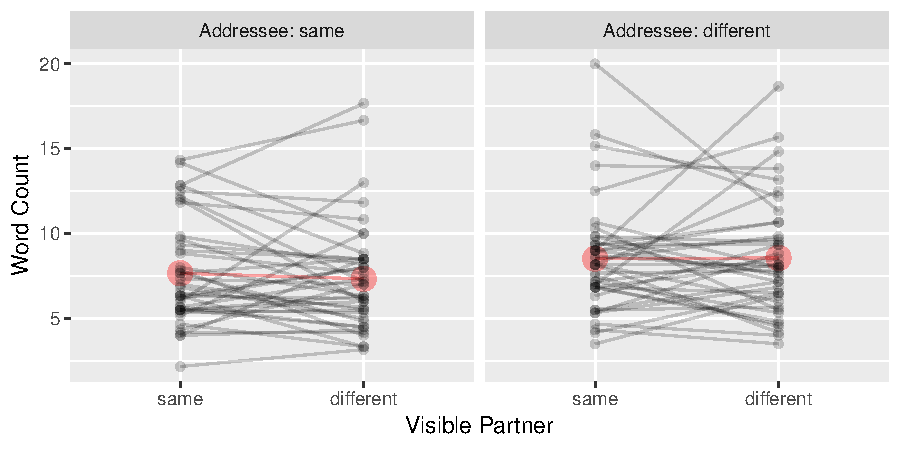
\includegraphics[width=.9\linewidth]{exp3/img/exp3-wc-plot.pdf}
\caption{\label{fig:orgaad91ed}
Word count for unconventional referent descriptions by Visible Partner and Addressee. Connected black points are individual participants and red points are grand means.}
\end{figure}

For the model of word count, we fit a generalized linear mixed-effects model with Poisson distribution function and log link.  The maximal model returned a singularity message, and so we fit a reduced model with a by-subject random intercepts, by-subject random slopes for \emph{Visible Partner}, \emph{Addressee}, and the \emph{Visible Partner-by-Addressee} interaction, with covariances constrained to zero; by-item random intercepts, by-item random slopes for \emph{Addressee}, and covariances constrained to zero. The data are shown in Figure~\ref{fig:orgaad91ed}.

There was a significant effect of \emph{Addressee} on word count, with longer descriptions given when the partner at test was different from the training partner,
\(M = 8.5\)  \((SD = 5.5)\),
compared to descriptions given to the same partner,
\(M = 7.5\)  \((SD = 4.7)\),
\(\beta = -0.26\), \(SE = 0.06\), Wald \(z = -4.48\), \(p < .001\).

There was little evidence for any effect of \emph{Visible Partner} on word count; 
for descriptions in the \emph{Different Partner} condition,
\(M = 7.9\)  \((SD = 5.4)\),
versus descriptions in the \emph{Same Partner} condition,
\(M = 8.1\)  \((SD = 4.9)\),
\(\beta = -0.01\), \(SE = 0.03\), Wald \(z = -0.30\), \(p = 0.762\).

Finally, there was little evidence for a \emph{Visible Partner-by-Addressee} interaction. When the visible partner was the same as in training, speakers produced descriptions that were on average 
0.9 
words longer for the new addressee; 
this effect was not significantly different from the case where the visible partner was different from the training partner, where speakers produced descriptions that were on average
1.2
words longer for the new addressee,
\(\beta = 0.01\), \(SE = 0.08\), Wald \(z = 0.19\), \(p = 0.850\).

\section*{General Discussion}
\label{sec:orga62f51b}
Over three experiments, we sought to test whether ordinary memory processes---as embodied in the encoding specificity principle \citep{tulvingthomson73}---influence the selection of information in the generation of referential descriptions. The basic logic of the experiments was to have speakers entrain on particular descriptions for referents in specific contexts, and then present the same referents in a context with different informational requirements but varying in similarity to the training context. The key prediction was that speakers' tendency to use the (no longer appropriate) entrained-upon description would vary as a function of the similarity between the training and test contexts. Support for this prediction was weak and inconsistent: no statistically reliable effect in Experiment~1, with a difference in means of less than 1\%; a statistically significant congruency effect in Experiment~2 (pre-registered one-tailed test, \(p =\)0.030), but with a difference of less than 5\%; and finally, a numerical difference of 5\% in Experiment~3, but in the wrong direction.

Despite limited overall support for the main prediction that training-test similarity would modulate misspecification rates, all three experiments show strong memory effects, inasmuch as speakers misspecified targets at high rates overall across all three experiments: 16\% in Experiment~1, 82\% in Experiment~2, and 60\% in Experiment~3.  These high misspecification rates indicate that speakers did retain information from training episodes; moreoever, the eye data from Experiment~2 indicated strong and detailed memory for the training display configurations, although the impact on speech was limited. Finally, these mostly null effects of memory are contrasted with positive evidence for a common ground effect in Experiment~3, where speakers lengthened descriptions of unconventional referents for new addressees. Taken together, these findings support the idea that speakers do maintain detailed representations about past referring episodes, but these representations have little role in the message generation process, even when the representations are related to the identity of an interacting conversational partner.  Instead, it appears that much of message generation is driven by coarse-grained memory representations that do not contain much more information than the identity of the target referent and the label given to it on previous occasions.

It is illustrative to consider these findings in relation to recent findings from comprehension. Episodic effects on comprehension have been studied in a similar paradigm, in terms of whether reference resolution is facilitated when listeners hear expressions repeated in the voice of the speaker who established the precedent. Although early experiments failed to find such facilitation \citep{barrkeysar02,metzingbrennan03}, it was eventually detected in later experiments that used more sensitive measures and larger samples \citep{brown-schmidt09prec}. A meta-analysis suggested these effects are likely to exist, but are small and fleeting \citep{kronmuller_barr_2015} especially when compared to the very large and reliable partner-independent effects. In short, abstract symbolic memory representations, such as the association between a referent and a referring expression, appear to have strong impacts on language processing, but the role of more detailed episodic representations appears marginal at best. That said, our findings for production are best viewed as limiting the explanatory scope of ordinary memory models, rather than as an overall rejection of this view. Our studies have only looked only at short-term memories formed within the confines of the laboratory, and perhaps repetition across a longer time frame could produce larger effects.

Another consideration is that across all experiments, we used experimenters as listeners rather than actual participants. One possibility is that because our experimenters were practiced at the task, back-and-forth interaction was more limited than it would be with uninformed listeners, and perhaps speakers attended less to the referring context than they would otherwise, thus forming impoverished representations. Against this interpretation, we note that we did find strong partner effects in Experiment~3 with the unconventional targets, which demonstrates that speakers were treating the two listeners as having different knowledge and did in fact encode information about the context. Furthermore, it could be argued that using real listeners could lead to weaker encoding of context, since they would be likely to produce more variable responses, respond with greater delay, and their relative unfamiliarity and uncertainty could distract attention from the displays onto the interaction itself.

Finally, we note that Experiment~3 replicates the main findings of the study by \cite{GannBarr2014} on referential precedents. As in that earlier study, there was no reliable evidence that speakers were less likely to continue using referential precedents when speaking to a new addressee than when continuing to speak to the old addressee. Similarly, we also found that speakers lengthened their descriptions of unconventional targets when speaking to a new addressee, supporting the assumption that speakers were indeed attending to common ground. Although these two findings appear to be in conflict, \cite{GannBarr2014} noted that the long descriptions that speakers give when describing unconventional targets provide speakers with a greater opportunity to incrementally adapt their description to meet an uninformed addressee's needs. Supporting this view, despite producing longer descriptions, speakers' onset latencies were no greater when they spoke to new addressees, which indicates that the extra content was not part of the original plan. Also, there was evidence that the length of speakers' utterances could be predicted by hesitation behaviors emitted by the addressee, again supporting the idea that the extra content is added incrementally.

The question of how speakers select information in language production remains one of the least studied, and thus, most mysterious aspects of language production. One point that scholars can agree on is that much of what speakers choose to say seems to be driven in large part by information availability, but the concept of `availability' remains a poor explanatory construct. While ordinary memory processes are inevitably involved, what they deliver up to production processes are largely abstract symbolic representations, which makes it unlikely that these processes serve as an effective proxy for common ground in everyday conversation.

\section*{Context}
\label{sec:org6c4624a}

The work presented in this paper was completed as part of Kieran J. O'Shea's PhD thesis, which was supervised by Dale J. Barr. While Barr and O'Shea discussed previous studies investigating memory effects in referential description, they realized that these studies had not completely de-confounded memory retrieval from message generation, and developed the current experiments in response. Caitlyn R. Martin worked as research assistant on the project.

\bibliography{refs_R.bib}
\end{document}
